% ------------------------------------------------------------------------------
% TYPO3 Version 10 LTS - What's New (English Version)
%
% @author	Michael Schams <schams.net>
% @license	Creative Commons BY-NC-SA 3.0
% @link		https://typo3.org/help/documentation/whats-new/
% @language	English
% ------------------------------------------------------------------------------

\section{In-depth Changes}
\begin{frame}[fragile]
	\frametitle{In-depth Changes}

	\begin{center}\huge{\color{typo3darkgrey}\textbf{In-depth Changes}}\end{center}
	\begin{center}\large{\textit{Improvements and new features for integrators and developers}}\end{center}

\end{frame}

% ------------------------------------------------------------------------------
% Feature | 78432 | Add log message for Switch User action

\begin{frame}[fragile]
	\frametitle{In-depth Changes}
	\framesubtitle{Backend User Switch}

	\begin{itemize}
		\item A log message is written if an admin user switches to another backend user:
	\end{itemize}

	\begin{figure}
		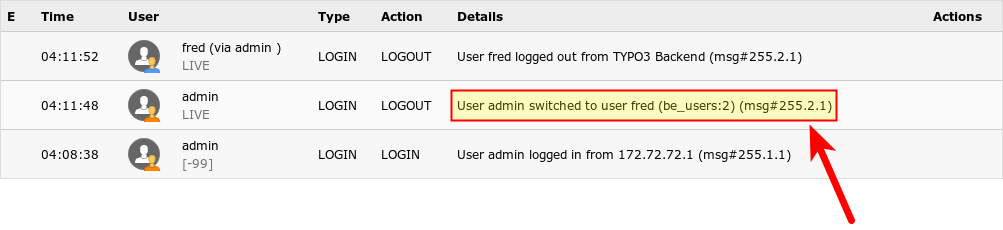
\includegraphics[width=0.90\linewidth]{InDepthChanges/78432-SwitchUserActionLogMessage.png}
	\end{figure}

\end{frame}

% ------------------------------------------------------------------------------
% Feature | 83734 | Add support for current page in configcache
% Breaking | 88564 | PageTSconfig setting TSFE.constants removed
% Breaking | 88657 | Popup configuration in FormEngine dropped

\begin{frame}[fragile]
	\frametitle{In-depth Changes}
	\framesubtitle{TypoScript Changes}

	\begin{itemize}
		\item TypoScript property \texttt{config.cache} now supports keyword
			"\texttt{current}" to refer to the current page. For example:\newline
			\smaller\texttt{config.cache.all = fe\_users:current}\normalsize

		\item The Page/User TSconfig setting \texttt{TSFE.constants} has been removed.

			\begin{itemize}\smaller
				\item[\ding{228}] Include TypoScript conditions in setup/constants and use a proper configuration in file \texttt{ext\_localconf.php}.
			\end{itemize}

		\item The following two options to configure the size of popup windows have been removed:

			\begin{itemize}
				\item \texttt{options.popupWindowSize}
				\item \texttt{options.rte.popupWindowSize}
			\end{itemize}

	\end{itemize}

\end{frame}

% ------------------------------------------------------------------------------
% Breaking | 88640 | Database field sys_template.nextLevel and TypoScript sublevel inheritance removed
% Task | 88755 | Remove POST option from typolink.addQueryString

\begin{frame}[fragile]
	\frametitle{In-depth Changes}
	\framesubtitle{TypoScript Changes}

	\begin{itemize}
		\item The database field \texttt{nextLevel} of the database table
			\texttt{sys\_template} has been removed.

			\begin{itemize}\smaller
				\item[\ding{228}] Replace the record (the UID is stored in the field \texttt{nextLevel}) with a condition to add TypoScript for subpages. For example: \texttt{[tree.level > 1]}
			\end{itemize}\normalsize

		\item The following values are \textbf{not allowed} anymore:

			\begin{itemize}\smaller
				\item \texttt{typolink.addQueryString.method = POST}
				\item \texttt{typolink.addQueryString.method = GET,POST}
				\item \texttt{typolink.addQueryString.method = POST,GET}
			\end{itemize}\normalsize

			\begin{itemize}\smaller
				\item[\ding{228}] Change the assignments in TypoScript, Fluid and PHP to \texttt{GET}.
			\end{itemize}\normalsize

	\end{itemize}

\end{frame}

% ------------------------------------------------------------------------------
% 87499 | Drop extensions "taskcenter" and "sys_action" from core

\begin{frame}[fragile]
	\frametitle{In-depth Changes}
	\framesubtitle{Task Center and \texttt{EXT:sys\_action}}

	\begin{itemize}

		\item The system extensions \texttt{EXT:taskcenter} and \texttt{EXT:sys\_action}
			have been removed from the core.

		\item They are now available as separate extensions from the
			\href{https://extensions.typo3.org/}{TER}
			and at
			\href{https://github.com/FriendsOfTYPO3}{GitHub}.

		\item The Dashboard replaces the Task Center and \texttt{EXT:sys\_action}.

	\end{itemize}

\end{frame}

% ------------------------------------------------------------------------------
% Feature | 89227 | Ask for email address while installing TYPO3

\begin{frame}[fragile]
	\frametitle{In-depth Changes}
	\framesubtitle{Administrator Email Address}

	\begin{columns}[T]
		\begin{column}{.04\textwidth}
		\end{column}
		\begin{column}{.38\textwidth}

			An email address can now be entered as part of the installation process.
			This address is used for the initial administrator backend user.

			\vspace{0.2cm}

			The same option exists in the Install Tool's Maintenance module
			\textbf{Create Administrative User}.

		\end{column}
		\begin{column}{.58\textwidth}
			\vspace{-0.3cm}
			\begin{figure}
				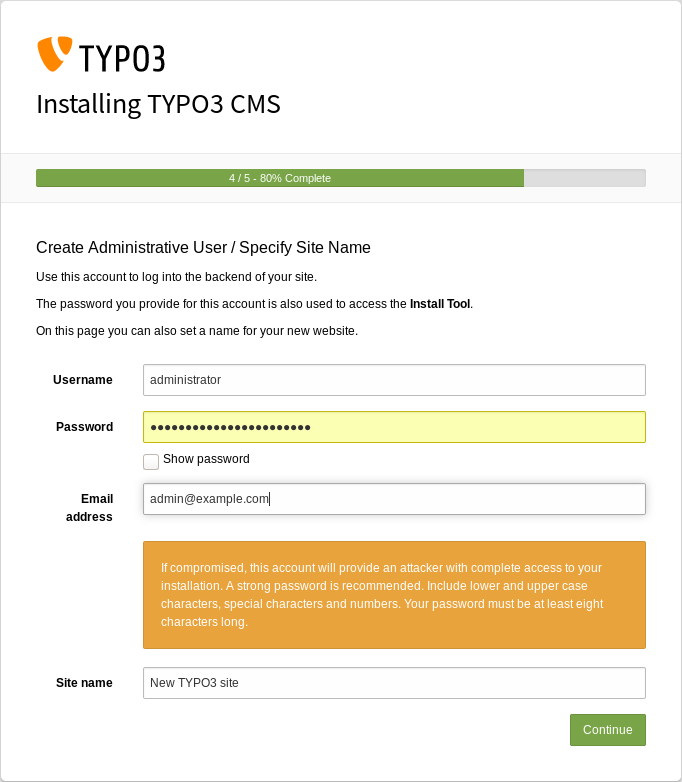
\includegraphics[width=0.70\linewidth]{InDepthChanges/89227-EmailAddressDuringInstallation.png}
			\end{figure}
		\end{column}
	\end{columns}

\end{frame}

% ------------------------------------------------------------------------------
% Breaking | 87583 | Remove obsolete APC Cache Backend implementation
% Breaking | 87558 | Consolidate extbase caches

\begin{frame}[fragile]
	\frametitle{In-depth Changes}
	\framesubtitle{Caches}

	% decrease font size for code listing
	\lstset{basicstyle=\tiny\ttfamily}

	\begin{itemize}
		\item Caching framework does not support the \texttt{ApcBackend} anymore

			\begin{itemize}\smaller
				\item[\ding{228}] Use \textbf{APCu} instead - note the "u".
			\end{itemize}
\begin{lstlisting}
OLD:
$GLOBALS['TYPO3_CONF_VARS']['SYS']['caching']['cacheConfigurations']['rootline']['backend'] =
\TYPO3\CMS\Core\Cache\Backend\ApcBackend::class;

NOW:
$GLOBALS['TYPO3_CONF_VARS']['SYS']['caching']['cacheConfigurations']['rootline']['backend'] =
\TYPO3\CMS\Core\Cache\Backend\ApcuBackend::class;
\end{lstlisting}

		\item Extbase caches \texttt{extbase\_reflection} and \texttt{extbase\_datamapfactory\_datamap}
			have been consolidated and are now available as a single cache named "\texttt{extbase}".

	\end{itemize}

\end{frame}

% ------------------------------------------------------------------------------
% Feature | 89229 | Cache Preset for Settings in Maintenance Area

\begin{frame}[fragile]
	\frametitle{In-depth Changes}
	\framesubtitle{Cache Storage Type}

	\begin{itemize}

		\item TYPO3 features a flexible caching system with a default configuration
			that is ideal for most use cases.
		\item The storage type can now be configured to fine-tune the caches and
			increase performance depending on the individual environment.

			\begin{itemize}
				\item Choose the \textbf{database} storage for a standard environment
					or if a network file system (NFS) is used for example.
				\item Choose the \textbf{file system} if a distributed database setup
					is used for example.
				\item Choose \textbf{custom cache settings} to configure the storage
					type for each cache independently.
			\end{itemize}

		\item For more complex installations, memory-based caches such as
			\href{https://redis.io/}{Redis}
			or
			\href{https://memcached.org/}{Memcached}
			should be considered.

	\end{itemize}

\end{frame}

% ------------------------------------------------------------------------------
% Feature | 89229 | Cache Preset for Settings in Maintenance Area

\begin{frame}[fragile]
	\frametitle{In-depth Changes}
	\framesubtitle{Cache Storage Type}

	Admin Tools \ding{223}\hspace{0.1cm}Settings \ding{223}\hspace{0.1cm}Configuration Presets \ding{223}\hspace{0.1cm}Cache Settings:

	\begin{figure}
		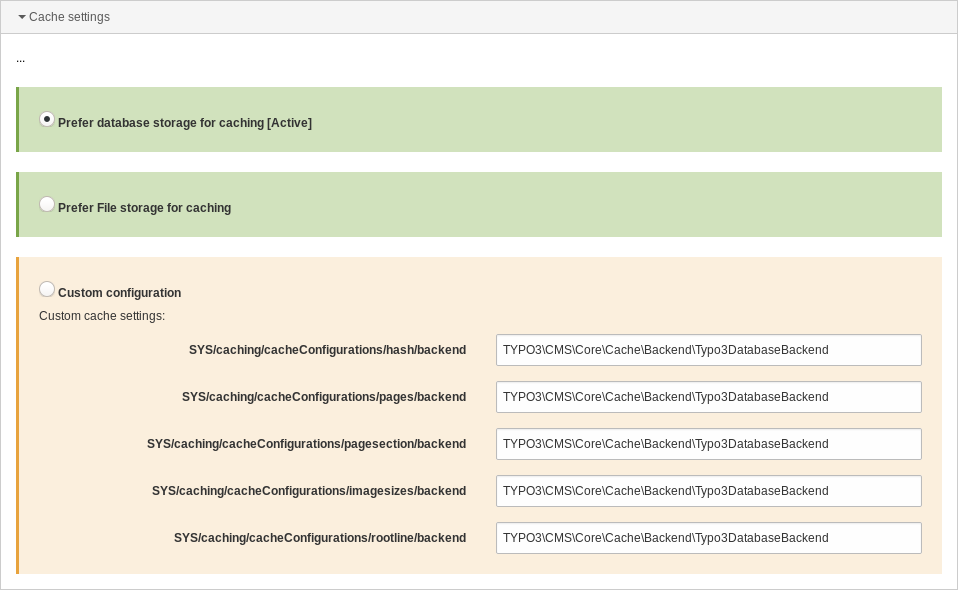
\includegraphics[width=0.70\linewidth]{InDepthChanges/89229a-CachePresetForSettingsInMaintenanceArea.png}
	\end{figure}

\end{frame}

% ------------------------------------------------------------------------------
% Feature | 89054 | Provide core cache frontends via dependency injection

\begin{frame}[fragile]
	\frametitle{In-Depth Changes}
	\framesubtitle{Cache Dependency Injection}

	% decrease font size for code listing
	\lstset{basicstyle=\tiny\ttfamily}

	\begin{itemize}
		\item Extension developers are encouraged to inject caches directly rather than using the CacheManager.
		\item This requires a few simple changes as shown below.

		\item \textbf{Previously:}
\begin{lstlisting}
class MyClass
{
  /**
   * @var TYPO3\CMS\Core\Cache\Frontend\FrontendInterface
   */
  private $cache;

  public function __construct()
  {
      $cacheManager = GeneralUtility::makeInstance(CacheManager::class);
      $this->cache = $cacheManager->getCache('my_cache');
  }
}
\end{lstlisting}

	\end{itemize}

\end{frame}

% ------------------------------------------------------------------------------
% Feature | 89054 | Provide core cache frontends via dependency injection

\begin{frame}[fragile]
	\frametitle{In-Depth Changes}
	\framesubtitle{Cache Dependency Injection}

	% decrease font size for code listing
	\lstset{basicstyle=\tiny\ttfamily}

	\begin{itemize}
		\item In \textbf{TYPO3 v10 LTS}, the class should look as follows:
\begin{lstlisting}
class MyClass
{
  /**
   * @var TYPO3\CMS\Core\Cache\Frontend\FrontendInterface
   */
  private $cache;

  public function __construct(FrontendInterface $cache)
  {
    $this->cache = $cache;
  }
}
\end{lstlisting}

	\end{itemize}

\end{frame}

% ------------------------------------------------------------------------------
% Feature | 89054 | Provide core cache frontends via dependency injection

\begin{frame}[fragile]
	\frametitle{In-Depth Changes}
	\framesubtitle{Cache Dependency Injection}

	% decrease font size for code listing
	\lstset{basicstyle=\tiny\ttfamily}

	\begin{itemize}
		\item ...and the following container service configuration is required:
\begin{lstlisting}
services:
  cache.my_cache:
    class: TYPO3\CMS\Core\Cache\Frontend\FrontendInterface
    factory: ['@TYPO3\CMS\Core\Cache\CacheManager', 'getCache']
    arguments: ['my_cache']

  MyClass:
    arguments:
      $cache: '@cache.my_cache'
\end{lstlisting}

	\end{itemize}

\end{frame}

% ------------------------------------------------------------------------------
% Deprecation | 88366 | Default caching framework cache names changed

\begin{frame}[fragile]
	\frametitle{In-Depth Changes}
	\framesubtitle{Caching Framework}

	% decrease font size for code listing
	\lstset{basicstyle=\tiny\ttfamily}

	\begin{itemize}
		\item The following caches have been renamed:

			\begin{itemize}\smaller
				\item \texttt{cache\_core} \textrightarrow\hspace{0.1cm}\texttt{core}
				\item \texttt{cache\_hash} \textrightarrow\hspace{0.1cm}\texttt{hash}
				\item \texttt{cache\_pages} \textrightarrow\hspace{0.1cm}\texttt{pages}
				\item \texttt{cache\_pagesection} \textrightarrow\hspace{0.1cm}\texttt{pagesection}
				\item \texttt{cache\_runtime} \textrightarrow\hspace{0.1cm}\texttt{runtime}
				\item \texttt{cache\_rootline} \textrightarrow\hspace{0.1cm}\texttt{rootline}
				\item \texttt{cache\_imagesizes} \textrightarrow\hspace{0.1cm}\texttt{imagesizes}
			\end{itemize}\normalsize

		\item New method to access the caches:
\begin{lstlisting}
OLD:
$cacheManager->getCache('cache_core').

NEW:
$cacheManager->getCache('core')
\end{lstlisting}

		\item The prefix \texttt{cf\_} has been removed from the database tables.
	\end{itemize}

\end{frame}

% ------------------------------------------------------------------------------
% Feature | 89090 | Reports for conflicting redirects

\begin{frame}[fragile]
	\frametitle{In-depth Changes}
	\framesubtitle{Conflicting Redirects}

	\begin{itemize}
		\item A new Symfony command has been introduced to detect redirects
			that conflict with page URLs.
		\item Execute the command in the CLI:\newline
			\smaller
				(optional parameter \texttt{-}\texttt{-site} limits the check to a specific site)
			\normalsize
	\end{itemize}

	\begin{figure}
		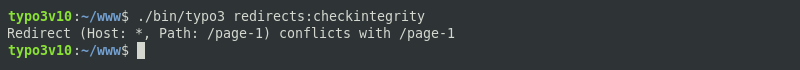
\includegraphics[width=0.90\linewidth]{InDepthChanges/89090a-ReportsForConflictingRedirects.png}
	\end{figure}

	\begin{itemize}
		\item The command is also available as a scheduler task:
	\end{itemize}

	\begin{figure}
		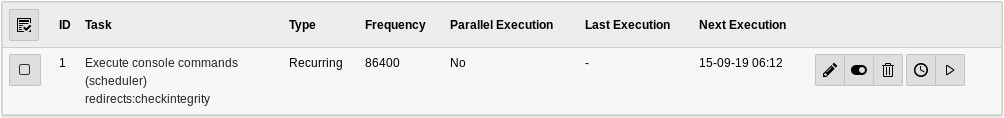
\includegraphics[width=0.90\linewidth]{InDepthChanges/89090b-ReportsForConflictingRedirects.png}
	\end{figure}

\end{frame}

% ------------------------------------------------------------------------------
% Feature | 89090 | Reports for conflicting redirects

\begin{frame}[fragile]
	\frametitle{In-depth Changes}
	\framesubtitle{Conflicting Redirects}

	\begin{itemize}
		\item A list of detected conflicting redirects can also be accessed in the Reports module:
	\end{itemize}

	\begin{figure}
		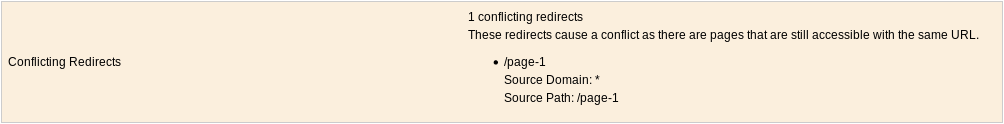
\includegraphics[width=0.90\linewidth]{InDepthChanges/89090c-ReportsForConflictingRedirects.png}
	\end{figure}

	\begin{itemize}
		\item
			\small\textbf{Note:}
				The command needs to be executed again to "reset" the list.
				Solving the issue (e.g. by removing the redirect) does not clear the list.
			\normalsize
	\end{itemize}

\end{frame}

% ------------------------------------------------------------------------------
% Feature | 89010 | Introduce Site Configuration for Distribution Packages

\begin{frame}[fragile]
	\frametitle{In-depth Changes}
	\framesubtitle{Distribution Packages}

	% decrease font size for code listing
	\lstset{basicstyle=\tiny\ttfamily}

	\begin{itemize}
		\item Distributions can now provide site configuration file(s).

		\item Create a directory/file in the distribution package as follows:\newline
			\texttt{Initialisation/Site/<siteIdentifier>/config.yaml}

		\item Similar to assets, which are moved to \texttt{fileadmin/},\newline
			site configurations are moved to the \texttt{config/} folder.

		\item If the target directory already exists, no change is made to the existing configuration.
	\end{itemize}

\end{frame}

% ------------------------------------------------------------------------------
% Feature | 88318 | Display Application Context in CLI

\begin{frame}[fragile]
	\frametitle{In-depth Changes}
	\framesubtitle{Application Context in CLI}

	\begin{itemize}
		\item The current Application Context is now shown next to the
			TYPO3 version number in CLI requests:
	\end{itemize}

	\begin{figure}
		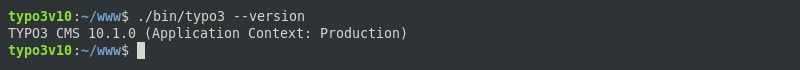
\includegraphics[width=0.90\linewidth]{InDepthChanges/88318-DisplayApplicationContextInCli.png}
	\end{figure}

\end{frame}

% ------------------------------------------------------------------------------
% Feature | 87525 | Add api=1 option in VimeoRenderer

\begin{frame}[fragile]
	\frametitle{In-depth Changes}
	\framesubtitle{Vimeo Video Rendering}

	% decrease font size for code listing
	\lstset{basicstyle=\smaller\ttfamily}

	\begin{itemize}
		\item The parameter \texttt{api=1} in Vimeo video URLs allows API interactions with the video player (e.g. adding buttons to control the video).
		\item Integrators can now set this parameter in two different ways.

		\begin{itemize}
			\item Using TypoScript:
\begin{lstlisting}
lib.contentElement.settings.media.additionalConfig.api = 1
\end{lstlisting}

			\item In Fluid using the Media-ViewHelper:
\begin{lstlisting}
<f:media
  file="{file}"
  alt="{file.properties.alternative}"
  title="{file.properties.title}"
  additionalConfig="{api: 1}"
/>
\end{lstlisting}

		\end{itemize}
	\end{itemize}

\end{frame}

% ------------------------------------------------------------------------------
% Feature | 86670 | Make default action in DragUploader adjustable

\begin{frame}[fragile]
	\frametitle{In-depth Changes}
	\framesubtitle{File Uploads}

	% decrease font size for code listing
	\lstset{basicstyle=\smaller\ttfamily}

	\begin{itemize}
		\item It is now possible to configure the default action when uploading files in the file list module using drag'n drop.
		\item User TSConfig:
\begin{lstlisting}
# Set default to replace:
options.file_list.uploader.defaultAction = replace

# Set default to rename:
options.file_list.uploader.defaultAction = rename

# Set default to cancel:
options.file_list.uploader.defaultAction = cancel
\end{lstlisting}

	\end{itemize}

\end{frame}

% ------------------------------------------------------------------------------
% Feature | 84250 | Separately enable / disable "Add media by URL" and "Select & upload files"

\begin{frame}[fragile]
	\frametitle{In-depth Changes}
	\framesubtitle{Media Element Buttons}

	% decrease font size for code listing
	\lstset{basicstyle=\tiny\ttfamily}

	\begin{itemize}
		\item Buttons \textbf{"Add media by URL"} and \textbf{"Select \& upload files"}
			can now be enabled/disabled independently from each other.
	\end{itemize}

	\begin{figure}
		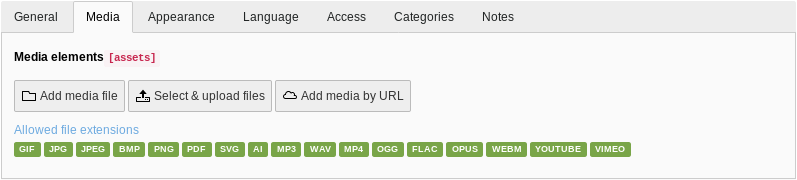
\includegraphics[width=0.75\linewidth]{InDepthChanges/84250-EnableDisableMediaButtons.png}
	\end{figure}

	\begin{itemize}
		\item The example below hides both buttons:
\begin{lstlisting}
$GLOBALS['TCA']['pages']['columns']['media']['config']['appearance'] = [
  'fileUploadAllowed' => false,
  'fileByUrlAllowed' => false,
];
\end{lstlisting}

	\end{itemize}

\end{frame}

% ------------------------------------------------------------------------------
% Feature | 88441 | Show configuration of USER_INT objects in adminpanel

\begin{frame}[fragile]
	\frametitle{In-depth Changes}
	\framesubtitle{Admin Panel}

	\begin{itemize}
		\item The Admin Panel features a new panel \textbf{USER\_INT} under the "Info" module.
	\end{itemize}

	\begin{figure}
		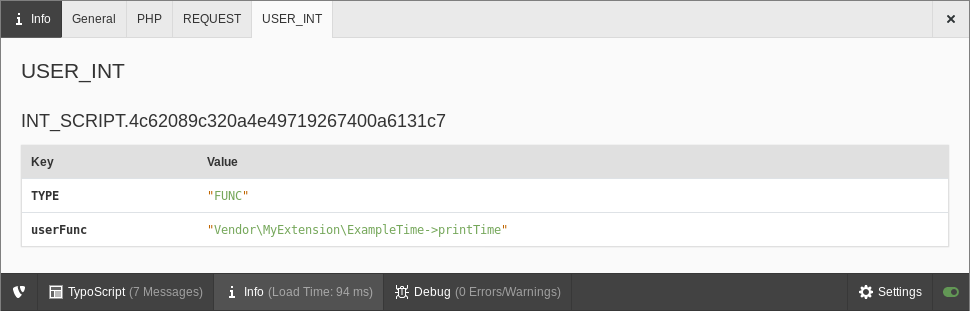
\includegraphics[width=0.90\linewidth]{InDepthChanges/88441-ShowUserIntObjectsInAdminPanel.png}
	\end{figure}

\end{frame}

% ------------------------------------------------------------------------------
% Feature | 89142 | Create site configuration if page is created on root level

\begin{frame}[fragile]
	\frametitle{In-depth Changes}
	\framesubtitle{Site Configuration}

	\begin{itemize}
		\item When a new page is created on the root level, a standard site
			configuration is automatically generated with it.
		\item As a result, a basic TYPO3 site can be set up quickly.
		\item The site configuration features:

			\begin{itemize}
				\item a pre-defined identifier (e.g. \texttt{autogenerated-1-c4ca4238a0})
				\item an entry point (e.g. \texttt{https://example.com/autogenerated-1})
				\item a default language (e.g. \texttt{English})
			\end{itemize}

	\end{itemize}

\end{frame}

% ------------------------------------------------------------------------------
% Feature | 85592 | Add site title configuration to sites module

\begin{frame}[fragile]
	\frametitle{In-depth Changes}
	\framesubtitle{Site Configuration}

	\begin{itemize}

		\item The site title can now be configured in
			\textbf{Site Configuration} $\rightarrow$ \textbf{Sites}.
		\item This lets integrators specify different site titles per language.
		\item The field in the template record is obsolete and has been marked as \textbf{deprecated}.
		\item The field \texttt{sys\_template.sitetitle} (database and TCA) will be removed in TYPO3 v11.
		\item The site title is used for the page title as well as for
			future \texttt{schema.org} integrations.
	\end{itemize}

\end{frame}

% ------------------------------------------------------------------------------
% Feature | 89398 | Support for environment variables in imports in site configurations

\begin{frame}[fragile]
	\frametitle{In-depth Changes}
	\framesubtitle{Site Configuration}

	% decrease font size for code listing
	\lstset{basicstyle=\tiny\ttfamily}

	\begin{itemize}

		\item It is now possible to use environment variables in imports of site configuration YAML files:
\begin{lstlisting}
imports:
  -
    resource: 'Env_%env("foo")%.yaml'
\end{lstlisting}

	\end{itemize}

\end{frame}

% ------------------------------------------------------------------------------
% Feature | 88102 | Frontend Login Form Via Fluid And Extbase

\begin{frame}[fragile]
	\frametitle{In-depth Changes}
	\framesubtitle{Frontend Login}

	\begin{itemize}

		\item TYPO3 v10 LTS now includes an Extbase-version of the frontend login functionality.
		\item This solution has a few advantages:

			\begin{itemize}
				\item Modify the templates more easily.
				\item Send out HTML-based password recovery emails.
				\item Adjust and modify validators to enforce password restrictions.
			\end{itemize}

		\item The new Extbase plugin is available out-of-the-box for new installations.
		\item Existing TYPO3 instances will continue to use the old templates.
		\item Integrators can switch between the "old" and the "new" plugin by using a feature toggle.

	\end{itemize}

\end{frame}

% ------------------------------------------------------------------------------
% Feature | 88110 | Felogin extbase password recovery

\begin{frame}[fragile]
	\frametitle{In-depth Changes}
	\framesubtitle{Frontend Login}

	\begin{itemize}

		\item A password recovery form has been added as part of the Extbase plugin.
		\item Users can request a password change and will receive an email with a link which redirects them to the form.
		\item Default password validation rules:

			\begin{itemize}
				\item \texttt{NotEmptyValidator} - passwords cannot be empty.
				\item \texttt{StringLengthValidator} - passwords must have a minimum length.
			\end{itemize}

	\end{itemize}

\end{frame}

% ------------------------------------------------------------------------------
% Feature | 88110 | Felogin extbase password recovery

\begin{frame}[fragile]
	\frametitle{In-depth Changes}
	\framesubtitle{Frontend Login}

	% decrease font size for code listing
	\lstset{basicstyle=\tiny\ttfamily}

	\begin{itemize}
		\item These validation rules can be customized.
		\item For example:
\begin{lstlisting}
plugin.tx_felogin_login {
  settings {
    passwordValidators {
      10 = TYPO3\CMS\Extbase\Validation\Validator\AlphanumericValidator
      20 {
        className = TYPO3\CMS\Extbase\Validation\Validator\StringLengthValidator
        options {
          minimum = 12
          maximum = 32
        }
      }
      30 = \Vendor\MyExtension\Validation\Validator\MyCustomPasswordPolicyValidator
    }
  }
}
\end{lstlisting}

	\end{itemize}

\end{frame}

% ------------------------------------------------------------------------------
% Feature | 89171 | Added possibility to have multiple sitemaps

\begin{frame}[fragile]
	\frametitle{In-depth Changes}
	\framesubtitle{Multiple Sitemaps}

	% decrease font size for code listing
	\lstset{basicstyle=\tiny\ttfamily}

	\begin{itemize}

		\item It is now possible to configure multiple sitemaps.
		\item Syntax:
\begin{lstlisting}
plugin.tx_seo {
  config {
    <sitemapType> {
      sitemaps {
        <unique key> {
          provider = TYPO3\CMS\Seo\XmlSitemap\RecordsXmlSitemapDataProvider
          config {
            ...
          }
        }
      }
    }
  }
}
\end{lstlisting}

	\end{itemize}

\end{frame}

% ------------------------------------------------------------------------------
% Feature | 86759 | Support nomodule attribute for JavaScript includes

\begin{frame}[fragile]
	\frametitle{In-depth Changes}
	\framesubtitle{HTML5 attribute \texttt{nomodule}}

	% decrease font size for code listing
	\lstset{basicstyle=\tiny\ttfamily}

	\begin{itemize}
		\item The HTML5 attribute \texttt{nomodule} is now supported when including JavaScript files in TypoScript.
\begin{lstlisting}
page.includeJSFooter.file = path/to/classic-file.js
page.includeJSFooter.file.nomodule = 1
\end{lstlisting}

		\item This attribute prevents a script from being executed in browsers that support module scripts.

		\item Read more about the standard in the
			\href{https://html.spec.whatwg.org/multipage/scripting.html#attr-script-nomodule}{specification}
			and about the concept of
			\href{https://hacks.mozilla.org/2015/08/es6-in-depth-modules/}{modules}.

	\end{itemize}

% <script type="module" src="path/to/file.js"></script>
% <script nomodule src="path/to/file/classic-file.js"></script>

\end{frame}

% ------------------------------------------------------------------------------
% Feature | 86918 | Add additional configuration for external link types in Linkvalidator

\begin{frame}[fragile]
	\frametitle{In-depth Changes}
	\framesubtitle{Link Validator}

	% decrease font size for code listing
	\lstset{basicstyle=\tiny\ttfamily}

	\begin{itemize}
		\item The Link Validator now supports additional configuration for external links.
		\item Values for \texttt{httpAgentUrl} and \texttt{httpAgentEmail} should be provided.
		\item Settings \texttt{headers}, \texttt{method} and \texttt{range} are advanced settings.
\begin{lstlisting}
mod.linkvalidator {
  linktypesConfig {
    external {
      httpAgentName = ...
      httpAgentUrl = ...
      httpAgentEmail = ...
      headers {
      }
      method = HEAD
      range = 0-4048
    }
  }
}
\end{lstlisting}

	\end{itemize}

\end{frame}

% ------------------------------------------------------------------------------
% Feature | 84990 | Add event for checking external links in RTE

\begin{frame}[fragile]
	\frametitle{In-depth Changes}
	\framesubtitle{Link Validator}

	\begin{itemize}
		\item Link Validator now marks broken \textbf{external} links in the RTE too.
		\item This feature was only available for internal links.
		\item It is recommended to run the Link Validator as a Scheduler task to regularly crawl for broken links.
	\end{itemize}

\end{frame}

% ------------------------------------------------------------------------------



% ------------------------------------------------------------------------------
% Important | 89992 | Use New TranslationServer
% Feature | 89526 | FeatureFlag: betaTranslationServer

\begin{frame}[fragile]
	\frametitle{In-depth Changes}
	\framesubtitle{Localization Management Platform}

	\begin{itemize}
		\item The SaaS solution "\href{https://crowdin.com/}{Crowdin}" is now used as
			the localization/translation management platform for TYPO3.
		\item We encourage everyone to participate and improve the localization.
		\item Crowdin can be used to translate language labels of the TYPO3 core
			as well as of TYPO3 extensions.
		\item Read more about the initiative in
			\href{https://typo3.org/community/teams/typo3-development/initiatives/localization-with-crowdin/}{this article}
			and in the
			\href{https://docs.typo3.org/m/typo3/reference-coreapi/master/en-us/ApiOverview/Internationalization/TranslationServer/Crowdin.html}{TYPO3 documentation}.
	\end{itemize}

	\begin{figure}
		
\includegraphics[width=0.40\linewidth]{InDepthChanges/crowdin-logo.png}
	\end{figure}

\end{frame}

% ------------------------------------------------------------------------------
% Feature | 90266 | Fluid-based templated emails

\begin{frame}[fragile]
	\frametitle{In-depth Changes}
	\framesubtitle{Fluid-based HTML Emails}

	% decrease font size for code listing
	\lstset{basicstyle=\smaller\ttfamily}

	\begin{itemize}
		\item TYPO3 now supports sending template-based HTML and plain-text emails.
		\item Emails are built by using the Fluid templating engine.
		\item Email templates can be customized by overwriting the paths to the template files:
\begin{lstlisting}
$GLOBALS['TYPO3_CONF_VARS']['MAIL']['templateRootPaths'][700] =
  'EXT:my_site_extension/Resources/Private/Templates/Email';

$GLOBALS['TYPO3_CONF_VARS']['MAIL']['layoutRootPaths'][700] =
  'EXT:my_site_extension/Resources/Private/Layouts';
\end{lstlisting}

	\end{itemize}

\end{frame}

% ------------------------------------------------------------------------------
% Feature | 90266 | Fluid-based templated emails

\begin{frame}[fragile]
	\frametitle{In-depth Changes}
	\framesubtitle{Fluid-based HTML Emails}

	\begin{itemize}
		\item Fluid-based templated emails are used for the following components for example:

			\begin{itemize}
				\item Install Tool test email (see example on the next slide).
				\item Workspace notification email on stage change.
				\item Notification email on backend user login.
			\end{itemize}

	\end{itemize}

\end{frame}

% ------------------------------------------------------------------------------
% Feature | 90266 | Fluid-based templated emails

\begin{frame}[fragile]
	\frametitle{In-depth Changes}
	\framesubtitle{Fluid-based HTML Emails}

	Test email sent from the Install Tool:

	\begin{figure}
		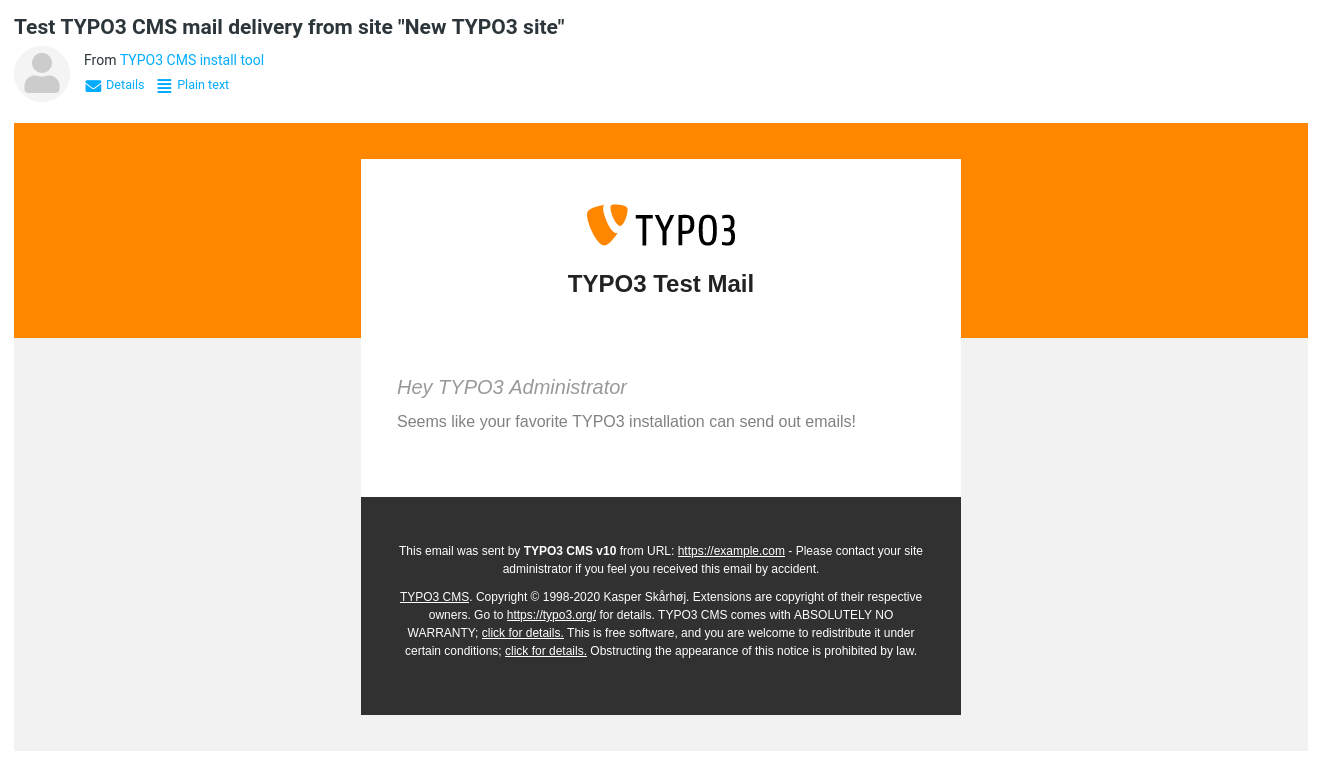
\includegraphics[width=0.8\linewidth]{InDepthChanges/90266-FluidBasedTemplatedEmails.png}
	\end{figure}

\end{frame}

% ------------------------------------------------------------------------------
% Feature | 88962 | Re-implement old PIDupinRootline TypoScript condition

\begin{frame}[fragile]
	\frametitle{In-depth Changes}
	\framesubtitle{TypoScript}

	% decrease font size for code listing
	\lstset{basicstyle=\smaller\ttfamily}

	\begin{itemize}
		\item The old \texttt{PIDupinRootline} condition has been re-implemented
			in TypoScript using the Symfony expression language.
		\item Old TypoScript condition syntax:
\begin{lstlisting}
[PIDupinRootline = 30]
  page.10.value = I'm on any subpage of page with UID 30.
[END]
\end{lstlisting}

		\item New TypoScript condition syntax:
\begin{lstlisting}
[30 in tree.rootLineParentIds]
  page.10.value = I'm on any subpage of page with UID 30.
[END]
\end{lstlisting}

	\end{itemize}

\end{frame}

% ------------------------------------------------------------------------------
% Feature | 90426 | Browser-native lazy loading for images

\begin{frame}[fragile]
	\frametitle{In-depth Changes}
	\framesubtitle{Lazy Loading for Images}

	% decrease font size for code listing
	\lstset{basicstyle=\smaller\ttfamily}

	\begin{itemize}
		\item The HTML attribute \texttt{loading} can now be set for \texttt{<img>}-tags.
		\item Browsers which support this feature won't load these images until they are in the viewport.
		\item The behavior can be modified by the following TypoScript constant:
\begin{lstlisting}
styles.content.image.lazyLoading = lazy
\end{lstlisting}

		\item Valid values are: \texttt{lazy} (default), \texttt{eager}, and \texttt{auto}.
		\item The Fluid \textit{Image-ViewHelper} also supports lazy loading now:
\begin{lstlisting}
<f:image src="{fileObject}" treatIdAsReference="true"
  loading="lazy" />
\end{lstlisting}

	\end{itemize}

\end{frame}

% ------------------------------------------------------------------------------
% Important | 89869 | Change lockIP default to disabled for both frontend and backend

\begin{frame}[fragile]
	\frametitle{In-depth Changes}
	\framesubtitle{Default values for \texttt{lockIP}/\texttt{lockIPv6}}

	% decrease font size for code listing
	\lstset{basicstyle=\smaller\ttfamily}

	\begin{itemize}
		\item The default values for \texttt{lockIP} settings have been changed.
		\item The following four system variables are now \textbf{disabled} by default:

			\begin{itemize}
				\item \texttt{[FE]['lockIP']}
				\item \texttt{[FE]['lockIPv6']}
				\item \texttt{[BE]['lockIP']}
				\item \texttt{[BE]['lockIPv6']}
			\end{itemize}

		\item The old default values ("\texttt{4}" for the backend and "\texttt{2}" for the frontend)
			caused problems for example for clients with IPv4 and IPv6 address support.

	\end{itemize}

\end{frame}

% ------------------------------------------------------------------------------
% Feature | 88147 | Add possibility to configure the path to sitemap xslFile

\begin{frame}[fragile]
	\frametitle{In-depth Changes}
	\framesubtitle{SEO: \texttt{Sitemap.xsl}}

	% decrease font size for code listing
	\lstset{basicstyle=\tiny\ttfamily}

	\begin{itemize}
		\item The default path to the file \texttt{Sitemap.xsl} of the system extension
			\texttt{EXT:seo} can be customized now:
\begin{lstlisting}
# Globally for all sitemaps:
plugin.tx_seo.config.xslFile = EXT:myext/Resources/Public/CSS/mySite.xsl

# For all sitemaps of a specific type:
plugin.tx_seo.config.<sitemapType>.sitemaps.xslFile = EXT:myext/Resources/Public/CSS/mySite.xsl

# For a specific sitemap:
plugin.tx_seo.config.<sitemapType>.sitemaps.<sitemap>.config.xslFile =
  EXT:myext/Resources/Public/CSS/mySite.xsl
\end{lstlisting}

		\item The default path reads:\newline
			\smaller
				\texttt{EXT:seo/Resources/Public/CSS/Sitemap.xsl}
			\normalsize

	\end{itemize}

\end{frame}

% ------------------------------------------------------------------------------
% Feature | 82062 | Progress for Reference Index update on CLI

\begin{frame}[fragile]
	\frametitle{In-depth Changes}
	\framesubtitle{Reference Index}

	% decrease font size for code listing
	\lstset{basicstyle=\tiny\ttfamily}

	\begin{itemize}
		\item Progress bars are shown for each database table during Reference Index update.
	\end{itemize}

	\begin{figure}
		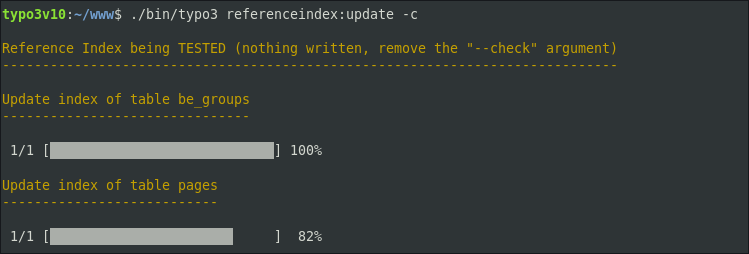
\includegraphics[width=0.85\linewidth]{InDepthChanges/82062-ProgressForReferenceIndexUpdateOnCli.png}
	\end{figure}

\end{frame}

% ------------------------------------------------------------------------------
% Feature | 59452 | scheduler:run command accepts multiple task options

\begin{frame}[fragile]
	\frametitle{In-depth Changes}
	\framesubtitle{Scheduler}

	% decrease font size for code listing
	\lstset{basicstyle=\tiny\ttfamily}

	\begin{itemize}
		\item Multiple tasks can be executed when using the option \texttt{-}\texttt{-}\texttt{task}
	\end{itemize}

	\begin{figure}
		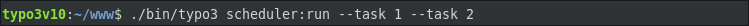
\includegraphics[width=0.85\linewidth]{InDepthChanges/59452a-MultipleTasksInSchedulerCommand.png}
	\end{figure}

	\begin{itemize}
		\item Verbose output can be enabled by \texttt{-}\texttt{v} and \texttt{-}\texttt{vv}
	\end{itemize}

	\begin{figure}
		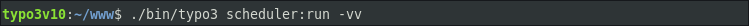
\includegraphics[width=0.85\linewidth]{InDepthChanges/59452b-MultipleTasksInSchedulerCommand.png}
	\end{figure}

\end{frame}

% ------------------------------------------------------------------------------
% Important | 18079 | pages.doktype restriction for frontend queries refined

\begin{frame}[fragile]
	\frametitle{In-depth Changes}
	\framesubtitle{Page Type Handling}

	\begin{itemize}
		\item TYPO3's internal handling of page types has changed.
		\item The option \texttt{pages.doktype} defines a numeric value that represents the type,
			e.g. standard page, folder, shortcut, link to external URL, etc.
		\item Pages of certain types (e.g. folder and recycler) were excluded when content was
			read from a specific page or records retrieved.
		\item This limitation has now been removed  and custom page doktypes with a number >200
			are now possible.
		\item Integrators and developers who have used page doktypes, e.g. in TypoScript,
			are advised to check if the previous behavior was misused and requires an update now.
	\end{itemize}

\end{frame}

% ------------------------------------------------------------------------------
% Feature | 90203 | Make workspace available in TypoScript conditions

\begin{frame}[fragile]
	\frametitle{In-depth Changes}
	\framesubtitle{Workspaces}

	% decrease font size for code listing
	\lstset{basicstyle=\smaller\ttfamily}

	\begin{itemize}
		\item A new expression language variable has been added: \texttt{workspace}.
		\item This variable can be used to match a given expression against common workspace parameters.
		\item Currently, the following parameters are supported:\newline
			\small
				\texttt{workspaceId}, \texttt{isLive}, and \texttt{isOffline}.
			\normalsize
		\item For example:
\begin{lstlisting}
[workspace.workspaceId === 3]
  # Current workspace ID is 3
[end]
\end{lstlisting}

	\end{itemize}

\end{frame}

% ------------------------------------------------------------------------------
% Important | 89555 | Workspace-related database records contain the proper Page ID

\begin{frame}[fragile]
	\frametitle{In-depth Changes}
	\framesubtitle{Workspaces}

	\begin{itemize}
		\item For many years, the TYPO3 core set \texttt{pid} to \texttt{-1} of unpublished records.
		\item TYPO3 now handles versioned records by validating the following three fields:

			\begin{itemize}
				\item \texttt{t3ver\_wsid} (the workspace ID the record is versioned in)
				\item \texttt{t3ver\_state} (the type of the versioned record)
				\item \texttt{t3ver\_oid} (the live version of a record)
			\end{itemize}

		\item Therefore, \texttt{pid=-1} is not required anymore.
		\item The Upgrade Wizard converts all \texttt{pid} fields of versioned records
			into the real \texttt{pid} values.
		\item New installations are not affected by this change.

	\end{itemize}

\end{frame}

% ------------------------------------------------------------------------------
% Deprecation | 91030 | Runtime-Activated Packages

\begin{frame}[fragile]
	\frametitle{In-depth Changes}
	\framesubtitle{Runtime-Activated Packages}

	\begin{itemize}
		\item The following global configuration option has been marked \textbf{deprecated}:\newline
			\smaller
				\texttt{\$GLOBALS['TYPO3\_CONF\_VARS']['EXT']['runtimeActivatedPackages']}
			\normalsize
		\item The use of runtime-activated extensions slows down a TYPO3 instance significantly.
		\item Integrators are adviced to take necessary steps, if such warnings apear
			in the deprecation log:\newline
			\begingroup
				\fontsize{8}{10}
				\texttt{Support for runtime activated packages will be removed in TYPO3 v11.0.}
			\endgroup

	\end{itemize}

\end{frame}

% ------------------------------------------------------------------------------
% Breaking | 88376 | Removed obsolete pageNotFound_handling settings

\begin{frame}[fragile]
	\frametitle{In-depth Changes}
	\framesubtitle{Page Not Found Handling}

	\begin{itemize}

		\item The following global TYPO3 settings have been removed:

			\begin{itemize}
				\item {\fontsize{7}{8}\selectfont\texttt{\$GLOBALS['TYPO3\_CONF\_VARS']['FE']['pageNotFound\_handling']}}
				\item {\fontsize{7}{8}\selectfont\texttt{\$GLOBALS['TYPO3\_CONF\_VARS']['FE']['pageNotFound\_handling\_statheader']}}
				\item {\fontsize{7}{8}\selectfont\texttt{\$GLOBALS['TYPO3\_CONF\_VARS']['FE']['pageNotFound\_handling\_accessdeniedheader']}}
				\item {\fontsize{7}{8}\selectfont\texttt{\$GLOBALS['TYPO3\_CONF\_VARS']['FE']['pageUnavailable\_handling']}}
				\item {\fontsize{7}{8}\selectfont\texttt{\$GLOBALS['TYPO3\_CONF\_VARS']['FE']['pageUnavailable\_handling\_statheader']}}
			\end{itemize}

			\begin{itemize}\smaller
				\item[\ding{228}] The Site Handling introduced in TYPO3 v9 replaces these settings.
			\end{itemize}\normalsize

	\end{itemize}

\end{frame}

% ------------------------------------------------------------------------------
% Important | 87980 | Page Is Being Generated Message Has Been Removed

\begin{frame}[fragile]
	\frametitle{In-depth Changes}
	\framesubtitle{Page Not Found Handling}

	\begin{itemize}

		\item The message "\textit{Page is being generated}" and the corresponding temporary
			HTTP 503 response have been removed.
	\end{itemize}

	\begin{figure}
		
\includegraphics[width=0.70\linewidth]{InDepthChanges/87980-PageIsBeingGenerated.png}
	\end{figure}

	\begin{itemize}
		\item Instead of offloading the work to wait for the final page content, concurrent
			requests now wait for the real page content to be rendered.
	\end{itemize}

\end{frame}

% ------------------------------------------------------------------------------
% Feature | 84262 | Update EXT:felogin to Extbase (long-term goal, not completed yet)
% Breaking | 88706 | Streamline felogin locallang keys
% Breaking | 88129 | Renamed felogin flexform fields

\begin{frame}[fragile]
	\frametitle{In-depth Changes}
	\framesubtitle{Frontend Login: Extbase}

	\begin{itemize}
		\item The frontend user login (\texttt{EXT:felogin}) has been converted to Extbase and Fluid.

		\item The following changes have been implemented:

		\begin{itemize}
			\item[\ding{202}] Prefix "\texttt{ll\_}" has been removed from locallang keys.

				\begin{itemize}
					\item[\ding{228}] Update your TypoScript if you have overwritten language labels and remove the prefix "\texttt{ll\_}" from your keys.
				\end{itemize}

			\item[\ding{203}] Existing FlexForm structure has been reworked.

				\begin{itemize}
					\item[\ding{228}] Execute the Upgrade Wizard to migrate the FlexForm values.
				\end{itemize}

		\end{itemize}

	\end{itemize}

\end{frame}

% ------------------------------------------------------------------------------
% Breaking | 88583 | Database field sys_language.static_lang_isocode removed
% Deprecation | 88567 | $GLOBALS['LOCAL_LANG']

\begin{frame}[fragile]
	\frametitle{In-depth Changes}
	\framesubtitle{Languages}

	\begin{itemize}
		\item ISO Codes:

			\begin{itemize}
				\item The unused database field \texttt{static\_lang\_isocode} has been removed.
				\item \texttt{EXT:static\_info\_tables} can be installed to reimplement functionality if required.
				\item Developers are advised to fetch all metadata for a language using the Site Configuration and the SiteLanguage API instead.
			\end{itemize}

		\item Language Files:

			\begin{itemize}
				\item Usage of the global array \texttt{\$GLOBALS[LOCAL\_LANG]} has been deprecated.
				\item The 2nd and 3rd arguments of \texttt{LanguageService->includeLLFile()} have been deprecated.
			\end{itemize}

	\end{itemize}

\end{frame}

% ------------------------------------------------------------------------------
% Feature | 88643 | New Mail API based on symfony/mailer and symfony/mime
% Breaking | 88643 | Removed Swiftmailerswiftmailer Dependency

\begin{frame}[fragile]
	\frametitle{In-Depth Changes}
	\framesubtitle{New Mail API}

	\begin{itemize}
		\item SwiftMailer has been superseded by more modern libraries:

			\begin{itemize}
				\item \texttt{symfony/mime} for creating mail messages
				\item \texttt{symfony/mailer} for sending emails
			\end{itemize}

		\item PHP function \texttt{mail()} is no longer supported.

			\begin{itemize}\smaller
				\item[\ding{228}] It is recommended to switch to \texttt{sendmail} or \texttt{smtp} instead.
			\end{itemize}\normalsize

		\item Custom SwiftMailer plugins or transports require a migration.

		\item See the \href{https://symfony.com/doc/current/mailer.html}{Symfony Documentation}
			for further details how to leverage the new Mail API capabilities.
	\end{itemize}

\end{frame}

% ------------------------------------------------------------------------------
% ...

\begin{frame}[fragile]
	\frametitle{In-Depth Changes}
	\framesubtitle{PSR Standards}

	\begin{itemize}
		\item TYPO3 v10 LTS follows these \href{https://www.php-fig.org/psr/}{PSR standards}:
			\vspace{0.2cm}
			\begin{itemize}
				\item PSR-0 / PSR-4\tabto{3.7cm}Autoloading
				\item PSR-1 / PSR-2\tabto{3.7cm}Coding Standards
				\item PSR-3\tabto{3.7cm}Logging
				\item PSR-7 / PSR-15 / PSR-17\tabto{3.7cm}HTTP Request / Response handling)
				\item PSR-11\tabto{3.7cm}Dependency Injection (Service Container)
				\item PSR-14\tabto{3.7cm}Event Dispatcher
				\item PSR-18\tabto{3.7cm}HTTP Client
			\end{itemize}

	\end{itemize}

\end{frame}

% ------------------------------------------------------------------------------
% Feature | 88799 | Use PSR-3 interface for logging

\begin{frame}[fragile]
	\frametitle{In-Depth Changes}
	\framesubtitle{PSR-3 Logging Interface}

	\begin{itemize}
		\item TYPO3's Logging Framework (in particular LogLevel and LogManager) now uses the
			\href{https://www.php-fig.org/psr/psr-3/}{PSR-3 Logger Interface}.

		\item PSR-3 is a standardized method that allows libraries to receive a
			\texttt{Psr\textbackslash
				Log\textbackslash
				LoggerInterface} object and to write logs to it in a simple and universal way.

			\item This lets developers use custom loggers and to interact with other
				logging systems.

	\end{itemize}

\end{frame}

% ------------------------------------------------------------------------------
% Feature | 84112 | Symfony dependency injection for core and Extbase

\begin{frame}[fragile]
	\frametitle{In-Depth Changes}
	\framesubtitle{PSR-11 Symfony's DependencyInjection}

	\begin{itemize}
		\item The package \texttt{symfony/dependency-injection} has been integrated
			and is used to manage system-wide dependency management and dependency
			injection for classes.

		\item This approach aims to replace the Extbase dependency injection
			container and object manager.

		\item Therefore, classes should be adjusted and avoid (whenever possible):

			\begin{itemize}\small
				\item \texttt{\textbackslash
					TYPO3\textbackslash
					CMS\textbackslash
					Extbase\textbackslash
					Object\textbackslash
					ObjectManager}
				\item \texttt{\textbackslash
					TYPO3\textbackslash
					CMS\textbackslash
					Core\textbackslash
					Utility\textbackslash
					GeneralUtility::makeInstance()}
			\end{itemize}\normalsize

	\end{itemize}

\end{frame}

% ------------------------------------------------------------------------------
% Feature | 84112 | Symfony dependency injection for core and Extbase

\begin{frame}[fragile]
	\frametitle{In-Depth Changes}
	\framesubtitle{PSR-11 Symfony's DependencyInjection}

	% decrease font size for code listing
	\lstset{basicstyle=\tiny\ttfamily}

	\begin{itemize}
		\item Configuration options include:

			\begin{itemize}
				\item Autowiring (see example below)
				\item Manual wiring
					(see \href{https://docs.typo3.org/c/typo3/cms-core/master/en-us/Changelog/10.0/Feature-84112-SymfonyDependencyInjectionForCoreAndExtbase.html}{change log})
				\item Advanced functionality
					(see \href{https://docs.typo3.org/c/typo3/cms-core/master/en-us/Changelog/10.0/Feature-84112-SymfonyDependencyInjectionForCoreAndExtbase.html}{change log})
			\end{itemize}
\begin{lstlisting}
# Configuration/Services.yaml
services:
  _defaults:
    autowire: true
    autoconfigure: true
    public: false

  Your\Namespace\:
    resource: '../Classes/*'
\end{lstlisting}

		\item See \href{https://symfony.com/doc/current/service_container.html}{Symfony documentation} for further details.

	\end{itemize}

\end{frame}

% ------------------------------------------------------------------------------
% Feature | 88769 | Introduce a generic EventDispatcher based on PSR-14
% Feature | 88770 | Add PSR-14 EventDispatcher logic based on DI

\begin{frame}[fragile]
	\frametitle{In-Depth Changes}
	\framesubtitle{PSR-14 Event Dispatching}

	\begin{itemize}
		\item A new "EventDispatcher" system has been added which aims to replace
			the hooks and Signal/Slots concepts.

		\item It is based on the \href{https://www.php-fig.org/psr/psr-14}{PSR-14 standard}
			which allows developers to inject logic into an application easily and consistently.

		\item PSR-14 consists of the following four components:

			\begin{itemize}
				\item An \textbf{EventDispatcher} object that is used to trigger an event.
				\item A \textbf{ListenerProvider} object that contains registered listeners for all events.
				\item One or multiple \textbf{Event} objects which are called from the TYPO3 core or extensions ("Emitter").
				\item One or multiple \textbf{Listeners} (usually in extensions and PHP packages) that are registered.
			\end{itemize}

% Short-Term goal is to deprecate SignalSlot dispatcher in TYPO3 v10,
% and migrate all signals to the EventDispatcher.

	\end{itemize}

\end{frame}

% ------------------------------------------------------------------------------
% Feature | 88769 | Introduce a generic EventDispatcher based on PSR-14
% Feature | 88770 | Add PSR-14 EventDispatcher logic based on DI

\begin{frame}[fragile]
	\frametitle{In-Depth Changes}
	\framesubtitle{PSR-14 Event Dispatching}

	% decrease font size for code listing
	\lstset{basicstyle=\tiny\ttfamily}

	Implementation example

	\begin{itemize}\smaller
		\item[\ding{202}] Add \texttt{event.listener} tag to the file \texttt{Configuration/Services.yaml}:
\begin{lstlisting}
services:
  Vendor\Example\EventListener\NullMailer:
    tags:
      - { name: event.listener, identifier: 'myListener', event: TYPO3\CMS\Core\Mail\Event\AfterMailerInitializationEvent, before: 'redirects, anotherIdentifier' }
\end{lstlisting}

		\item[\ding{203}] Implement your event object:
\begin{lstlisting}
namespace Vendor\Example\EventListener;

class NullMailer
{
  public function __invoke(AfterMailerInitializationEvent $event): void
  {
    $event->getMailer()->injectMailSettings(['transport' => 'null']);
  }
}
\end{lstlisting}

	\end{itemize}\normalsize

\end{frame}

% ------------------------------------------------------------------------------
% Feature | 88769 | Introduce a generic EventDispatcher based on PSR-14
% Feature | 88770 | Add PSR-14 EventDispatcher logic based on DI

\begin{frame}[fragile]
	\frametitle{In-Depth Changes}
	\framesubtitle{PSR-14 Event Dispatching}

	% decrease font size for code listing
	\lstset{basicstyle=\tiny\ttfamily}

	\begin{itemize}
		\item List of available Event Listeners can be accessed in the backend:\newline
			\smaller
				(requires system extension \texttt{EXT:lowlevel})
			\normalsize
	\end{itemize}

	\begin{figure}
		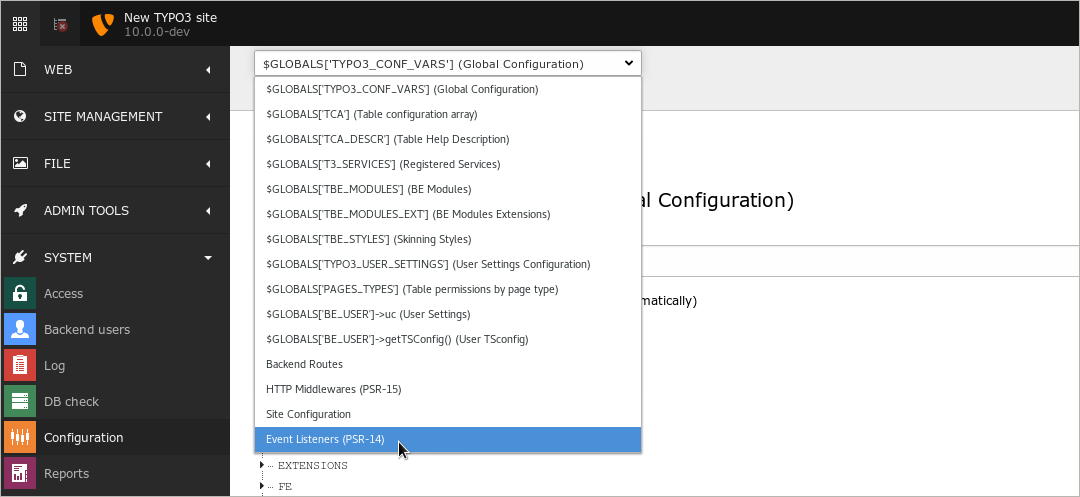
\includegraphics[width=0.70\linewidth]{InDepthChanges/88770-PSR14-EventDispatcher.png}
	\end{figure}

\end{frame}

% ------------------------------------------------------------------------------
% Feature | 88769 | Introduce a generic EventDispatcher based on PSR-14
% Feature | 88770 | Add PSR-14 EventDispatcher logic based on DI

\begin{frame}[fragile]
	\frametitle{In-Depth Changes}
	\framesubtitle{PSR-14 Event Dispatching}

	% decrease font size for code listing
	\lstset{basicstyle=\tiny\ttfamily}

	\begin{itemize}
		\item Best practices:

			\begin{itemize}
				\item Add only one Listener per PHP class and use \texttt{\_\_invoke()} as the method name.
				\item Add "\texttt{Event}" suffix to the class name when creating a new Event PHP class.
				\item Move the Event PHP class file to an appropriate folder e.g. \texttt{Classes/Database/Event}.
				\item Use dependency injection in form of a constructor argument to receive the
					EventDispatcher object if possible.
			\end{itemize}

		\item Additional note:\newline
			\small
				Events provided by the TYPO3 core follow TYPO3's deprecation policy, except for its constructor
				arguments which may vary.
			\normalsize

	\end{itemize}

\end{frame}

% ------------------------------------------------------------------------------
% Feature | 90265 | Show dispatched Events in Admin Panel

\begin{frame}[fragile]
	\frametitle{In-Depth Changes}
	\framesubtitle{PSR-14 Events in Admin Panel}

	\begin{itemize}
		\item The Admin Panel shows all PSR-14 events that have been dispatched in the current request.
	\end{itemize}

	\begin{figure}
		
\includegraphics[width=0.85\linewidth]{InDepthChanges/90265-ShowDispatchedEventsInAdminPanel.png}
	\end{figure}

\end{frame}

% ------------------------------------------------------------------------------
% Feature | 89018 | Provide implementation for PSR-17 HTTP Message Factories

\begin{frame}[fragile]
	\frametitle{In-Depth Changes}
	\framesubtitle{PSR-17 HTTP Message Factories}

	\begin{itemize}
		\item The \href{https://www.php-fig.org/psr/psr-17/}{PSR-17}
			HTTP Message Factories implementation has been added.
		\item HTTP Message Factory interfaces should be used as dependencies for
			request handlers or services that create PSR-7 message objects.
		\item PSR-17 consists of six factory interfaces:

			\begin{itemize}\smaller
				\item \texttt{\textbackslash
					Psr\textbackslash
					Http\textbackslash
					Message\textbackslash
					RequestFactoryInterface}
				\item \texttt{\textbackslash
					Psr\textbackslash
					Http\textbackslash
					Message\textbackslash
					ResponseFactoryInterface}
				\item \texttt{\textbackslash
					Psr\textbackslash
					Http\textbackslash
					Message\textbackslash
					ServerRequestFactoryInterface}
				\item \texttt{\textbackslash
					Psr\textbackslash
					Http\textbackslash
					Message\textbackslash
					StreamFactoryInterface}
				\item \texttt{\textbackslash
					Psr\textbackslash
					Http\textbackslash
					Message\textbackslash
					UploadedFileFactoryInterface}
				\item \texttt{\textbackslash
					Psr\textbackslash
					Http\textbackslash
					Message\textbackslash
					UriFactoryInterface}

			\end{itemize}\normalsize

		\item See
			\href{https://docs.typo3.org/c/typo3/cms-core/master/en-us/Changelog/10.1/Feature-89018-ProvideImplementationForPSR-17HTTPMessageFactories.html}{documentation}
			for a code example.

	\end{itemize}

\end{frame}

% ------------------------------------------------------------------------------
% Feature | 89216 | PSR-18 HTTP Client Implementation

\begin{frame}[fragile]
	\frametitle{In-Depth Changes}
	\framesubtitle{PSR-18 HTTP Client}

	\begin{itemize}
		\item The \href{https://www.php-fig.org/psr/psr-18/}{PSR-18}
			HTTP Client implementation has been added.
		\item It lets developers generate HTTP requests based on PSR-7
			message objects without relying on a specific HTTP client implementation.
		\item It does not replace the existing \href{http://guzzlephp.org/}{Guzzle}
			wrapper, but provides a more generic alternative.
		\item PSR-18 consists of a client interface and three exception interfaces:

			\begin{itemize}\smaller
				\item \texttt{\textbackslash
					Psr\textbackslash
					Http\textbackslash
					Client\textbackslash
					ClientInterface}
				\item \texttt{\textbackslash
					Psr\textbackslash
					Http\textbackslash
					Client\textbackslash
					ClientExceptionInterface}
				\item \texttt{\textbackslash
					Psr\textbackslash
					Http\textbackslash
					Client\textbackslash
					NetworkExceptionInterface}
				\item \texttt{\textbackslash
					Psr\textbackslash
					Http\textbackslash
					Client\textbackslash
					RequestExceptionInterface}
			\end{itemize}\normalsize

		\item See
			\href{https://docs.typo3.org/c/typo3/cms-core/master/en-us/Changelog/10.1/Feature-89216-PSR-18HTTPClientImplementation.html}{documentation}
			for a code example.

	\end{itemize}

\end{frame}

% ------------------------------------------------------------------------------
% Breaking | 88182 | jsfunc.inline.js has been dropped
% Breaking | 88427 | jsfunc.evalfield.js has been removed
% Breaking | 88667 | Removed additionalJavaScriptSubmit from FormEngine
% Deprecation | 88433 | Deprecate top.openUrlInWindow

\begin{frame}[fragile]
	\frametitle{In-Depth Changes}
	\framesubtitle{JavaScript Options and Functions}

	\begin{itemize}
		\item The following JavaScript files have been removed:

			\begin{itemize}
				\item \texttt{jsfunc.inline.js}
				\item \texttt{jsfunc.evalfield.js}
			\end{itemize}

			\begin{itemize}\smaller
				\item[\ding{228}] Use \texttt{TYPO3/CMS/Backend/FormEngineValidation} instead.
			\end{itemize}\normalsize

		\item Additional submit handlers could previously be added by the option \texttt{additionalJavaScriptSubmit}.
			This option has been removed.

			\begin{itemize}\smaller
				\item[\ding{228}] Create and register an AMD module instead.
			\end{itemize}\normalsize

		\item The global JavaScript function \texttt{top.openUrlInWindow()} has been marked deprecated.

	\end{itemize}

\end{frame}

% ------------------------------------------------------------------------------
% Breaking | 88411 | TBE_EDITOR.typo3form removed
% Deprecation | 88432 | Replaced md5js with an AMD module
% Deprecation | 88428 | top.rawurlencode and top.str_replace
% Deprecation | 88651 | Replace TYPO3/CMS/Backend/SplitButtons with TYPO3/CMS/Backend/DocumentSaveActions

\begin{frame}[fragile]
	\frametitle{In-Depth Changes}
	\framesubtitle{JavaScript Options and Functions}

	\begin{itemize}

		\item The global object \texttt{TBE\_EDITOR.typo3form} and its backward layers \texttt{typo3FormFieldSet}
			and \texttt{typo3FormFieldGet} have been removed.

		\item File \texttt{md5.js} has been marked deprecated.

			\begin{itemize}\smaller
				\item[\ding{228}] Load the AMD module \texttt{TYPO3/CMS/Backend/Hashing/Md5} via RequireJS instead.
			\end{itemize}\normalsize

		\item The following global JavaScript functions have been marked deprecated:

		\begin{itemize}
			\item \texttt{top.rawurlencode()}
			\item \texttt{top.str\_replace()}
		\end{itemize}

		\item Module \texttt{TYPO3/CMS/Backend.SplitButtons} has been deprecated.

			\begin{itemize}\smaller
				\item[\ding{228}] Use \texttt{TYPO3/CMS/Backend/DocumentSaveActions} instead.
			\end{itemize}\normalsize

 	\end{itemize}

\end{frame}

% ------------------------------------------------------------------------------
% Important | 87894 | Removed PHP Dependency algo26-matthiasidna-convert

\begin{frame}[fragile]
	\frametitle{In-Depth Changes}
	\framesubtitle{UTF-8-based Domains}

	\begin{itemize}
		\item PHP has native functions to convert domains from UTF-8 into IDNA ASCII form (“punicode”),
			for example \href{https://www.php.net/manual/en/function.idn-to-ascii.php}{idn\_to\_ascii()}.

		\item These can be used directly if the PHP extension
			"\href{https://www.php.net/manual/en/book.intl.php}{intl}" is installed.

		\item If the PHP extension is not installed, the package \texttt{symfony/polyfill-intl-idn}
			provides the functions now.

		\item Previously, the package \texttt{algo26-matthias/idna-convert} was used which has been removed now.

	\end{itemize}

\end{frame}

% ------------------------------------------------------------------------------
% Feature | 87665 | Introduce BitSet class

\begin{frame}[fragile]
	\frametitle{In-Depth Changes}
	\framesubtitle{BitSet Class}

	% decrease font size for code listing
	\lstset{basicstyle=\tiny\ttfamily}

	\begin{itemize}
		\item New class has been introduced to efficiently handle boolean flags:\newline
			\texttt{TYPO3\textbackslash
				CMS\textbackslash
				Core\textbackslash
				Type\textbackslash
				BitSet}

		\item For example:
\begin{lstlisting}
define('PERMISSIONS_NONE', 0b0); // 0
define('PERMISSIONS_PAGE_SHOW', 0b1); // 1
define('PERMISSIONS_PAGE_EDIT', 0b10); // 2
define('PERMISSIONS_PAGE_DELETE', 0b100); // 4
define('PERMISSIONS_PAGE_NEW', 0b1000); // 8
define('PERMISSIONS_CONTENT_EDIT', 0b10000); // 16
define('PERMISSIONS_ALL', 0b11111); // 31

$bitSet = new \TYPO3\CMS\Core\Type\BitSet(PERMISSIONS_PAGE_SHOW | PERMISSIONS_PAGE_NEW);
$bitSet->get(PERMISSIONS_PAGE_SHOW); // true
$bitSet->get(PERMISSIONS_CONTENT_EDIT); // false
\end{lstlisting}

	\end{itemize}

\end{frame}

% ------------------------------------------------------------------------------
% Important | 87516 | Remove Core HTTP Request Handler Interface

\begin{frame}[fragile]
	\frametitle{In-Depth Changes}
	\framesubtitle{Request Handler}

	\begin{itemize}
		\item The following internal interface has been removed
			in favor of PSR-15 request handler and middleware interfaces:\newline
			\texttt{TYPO3\textbackslash
				CMS\textbackslash
				Core\textbackslash
				Http\textbackslash
				RequestHandlerInterface}

	\end{itemize}

\end{frame}

% ------------------------------------------------------------------------------
% Breaking | 88687 | Configure extbase request handlers via PHP

\begin{frame}[fragile]
	\frametitle{In-Depth Changes}
	\framesubtitle{Request Handler}

	% decrease font size for code listing
	\lstset{basicstyle=\tiny\ttfamily}

	\begin{itemize}
		\item The configuration of Extbase request handlers is no longer possible with TypoScript.

		\smaller\textbf{Old} method in TypoScript:\normalsize
\begin{lstlisting}
config.tx_extbase {
  mvc {
    requestHandlers {
      Vendor\Example\Mvc\Web\FrontendRequestHandler = Vendor\Example\Mvc\Web\FrontendRequestHandler
    }
  }
}
\end{lstlisting}

		\smaller\textbf{New} method in file \texttt{Configuration/Extbase/RequestHandlers.php}:\normalsize
\begin{lstlisting}
<?php
declare(strict_types = 1);

return [
  \Vendor\Example\Mvc\Web\FrontendRequestHandler::class,
];
\end{lstlisting}

	\end{itemize}

\end{frame}

% ------------------------------------------------------------------------------
% Deprecation | 87550 | Use controller classes when registering plugins/modules

\begin{frame}[fragile]
	\frametitle{In-Depth Changes}
	\framesubtitle{Extbase and Fluid}

	% decrease font size for code listing
	\lstset{basicstyle=\tiny\ttfamily}

	\begin{itemize}
		\item Registering plugins/modules require fully-qualified class names now

			\begin{itemize}\smaller
				\item \texttt{\textbackslash
					TYPO3\textbackslash
					CMS\textbackslash
					Extbase\textbackslash
					Utility\textbackslash
					ExtensionUtility::configurePlugin()}
				\item \texttt{\textbackslash
					TYPO3\textbackslash
					CMS\textbackslash
					Extbase\textbackslash
					Utility\textbackslash
					ExtensionUtility::registerModule()}
			\end{itemize}\normalsize

		\item Also omit vendor name in the extension name (first argument).

			\begin{itemize}\smaller
				\item[\ding{228}] Use "\texttt{ExampleBlog}" instead of "\texttt{Vendor.ExampleBlog}".
			\end{itemize}

		\item For example:
\begin{lstlisting}
\TYPO3\CMS\Extbase\Utility\ExtensionUtility::configurePlugin(
  'ExampleBlog', // previously: 'Vendor.ExampleBlog'
  'pi1',
  [
    \Vendor\Example\Controller\BlogController::class => 'list,update,delete'
  ],
  [
    \Vendor\Example\Controller\BlogController::class => 'list,update,delete'
  ]
);
\end{lstlisting}

	\end{itemize}

\end{frame}

% ------------------------------------------------------------------------------
% Breaking | 87627 | Remove Property extensionName of AbstractController

\begin{frame}[fragile]
	\frametitle{In-Depth Changes}
	\framesubtitle{Extbase and Fluid}

	\begin{itemize}
		\item Property \texttt{extensionName} of AbstractController has been removed.

			\begin{itemize}\smaller
				\item[\ding{228}] Use \texttt{\textbackslash
					TYPO3\textbackslash
					CMS\textbackslash
					Extbase\textbackslash
					Mvc\textbackslash
					Request::getControllerExtensionName()} instead.
			\end{itemize}\normalsize

	\end{itemize}

\end{frame}

% ------------------------------------------------------------------------------
% Feature | 87457 | Use symfony/propertyinfo to gather doc block information

\begin{frame}[fragile]
	\frametitle{In-Depth Changes}
	\framesubtitle{Extbase and Fluid}

	% decrease font size for code listing
	\lstset{basicstyle=\tiny\ttfamily}

	\begin{itemize}
		\item Extbase models now support non fully-qualified class names in DocBlocks.
\begin{lstlisting}
use TYPO3\CMS\Extbase\Persistence\ObjectStorage;
use ExtbaseTeam\BlogExample\Domain\Model\Comment;

class Post
{
  /**
   * @var ObjectStorage<Comment>
   */
  public $comments;
}
\end{lstlisting}

	\end{itemize}

\end{frame}

% ------------------------------------------------------------------------------
% Breaking | 87957 | Validators are not registered automatically in Extbase anymore

\begin{frame}[fragile]
	\frametitle{In-Depth Changes}
	\framesubtitle{Extbase and Fluid}

	% decrease font size for code listing
	\lstset{basicstyle=\tiny\ttfamily}

	\begin{itemize}
		\item Validators are not registered automatically in Extbase anymore.
		\item For a model named
			\small\texttt{Vendor\textbackslash
				Example\textbackslash
				Domain\textbackslash
				Model\textbackslash
				Blog}\normalsize,\newline
			Extbase automatically used the validator
			\small\texttt{Vendor\textbackslash
				Example\textbackslash
				Domain\textbackslash
				Validator\textbackslash
				BlogValidator}\normalsize

		\item Validators need to be registered manually now:
\begin{lstlisting}
use Vendor\Example\Domain\Model\Blog;
use TYPO3\CMS\Extbase\Annotation as Extbase;
use TYPO3\CMS\Extbase\Mvc\Controller\ActionController;

class BlogController extends ActionController
{
  /**
   * @Extbase\Validate(param="blog", validator="Vendor\Example\Domain\Validator\BlogValidator")
   */
  public function showAction(Blog $blog)
  {
    // ...
  }
}
\end{lstlisting}

	\end{itemize}

\end{frame}

% ------------------------------------------------------------------------------
% Breaking | 87594 | Harden Extbase

\begin{frame}[fragile]
	\frametitle{In-Depth Changes}
	\framesubtitle{Extbase and Fluid}

	% decrease font size for code listing
	\lstset{basicstyle=\smaller\ttfamily}

	\begin{itemize}
		\item Class files now feature the "strict types" mode and type hints for scalars
\begin{lstlisting}
<?php
declare(strict_types=1);
\end{lstlisting}

		% Method signatures in Extbase classes have been updated.
		\item This results in fatal PHP errors if the method signatures in custom
			extensions are not compatible with the interfaces and/or parent classes.

		\item See \href{https://forge.typo3.org/issues/87594}{forge \#87594}
			for a complete list of files and their changes.

		\item This task is still work in progress and further changes will be made.

	\end{itemize}

\end{frame}

% ------------------------------------------------------------------------------
% Feature | 88995 | Calling registerPlugin with vendor name

\begin{frame}[fragile]
	\frametitle{In-Depth Changes}
	\framesubtitle{Extbase and Fluid}

	% decrease font size for code listing
	\lstset{basicstyle=\smaller\ttfamily}

	\begin{itemize}
		\item Omit the vendor name when registering plugins with\newline
			\smaller
				\texttt{\textbackslash
					TYPO3\textbackslash
					CMS\textbackslash
					Extbase\textbackslash
					Utility\textbackslash
					ExtensionUtility::registerPlugin()}
			\normalsize

		\item For example, use "\texttt{Form}" instead of "\texttt{TYPO3.CMS.Form}"\newline
			\small(first argument)\normalsize
\begin{lstlisting}
\TYPO3\CMS\Extbase\Utility\ExtensionUtility::registerPlugin(
  'Form',
  'Formframework',
  'Form',
  'content-form',
);
\end{lstlisting}

	\end{itemize}

\end{frame}

% ------------------------------------------------------------------------------
% Feature | 89870 | New PSR-14 Events for Extbase-related signals

\begin{frame}[fragile]
	\frametitle{In-Depth Changes}
	\framesubtitle{Extbase and Fluid}

	% decrease font size for code listing
	\lstset{basicstyle=\tiny\ttfamily}

	\begin{itemize}
		\item The following PSR-14-based events have been introduced for Extbase-related signals:
\begin{lstlisting}
TYPO3\CMS\Extbase\Event\Mvc\AfterRequestDispatchedEvent
TYPO3\CMS\Extbase\Event\Mvc\BeforeActionCallEvent
TYPO3\CMS\Extbase\Event\Persistence\AfterObjectThawedEvent
TYPO3\CMS\Extbase\Event\Persistence\ModifyQueryBeforeFetchingObjectDataEvent
TYPO3\CMS\Extbase\Event\Persistence\ModifyResultAfterFetchingObjectDataEvent
TYPO3\CMS\Extbase\Event\Persistence\EntityAddedToPersistenceEvent
TYPO3\CMS\Extbase\Event\Persistence\EntityFinalizedAfterPersistenceEvent
TYPO3\CMS\Extbase\Event\Persistence\EntityUpdatedInPersistenceEvent
TYPO3\CMS\Extbase\Event\Persistence\EntityRemovedFromPersistenceEvent
TYPO3\CMS\Extbase\Event\Persistence\EntityPersistedEvent
\end{lstlisting}

		\item Existing signals have been replaced and should not be used anymore.

	\end{itemize}

\end{frame}

% ------------------------------------------------------------------------------
% Breaking | 87623 | Replace config.persistence.classes typoscript configuration (1)

\begin{frame}[fragile]
	\frametitle{In-Depth Changes}
	\framesubtitle{Extbase and Fluid - Class Mapping}

	% decrease font size for code listing
	\lstset{basicstyle=\tiny\ttfamily}

	\begin{itemize}
		\item Persistence related class mapping using TypoScript is no longer supported:
\begin{lstlisting}
config.tx_example_blog {
  persistence {
    classes {
      Vendor\Example\Domain\Model\Author {
        mapping {
          tableName = fe_users
          columns.name.mapOnProperty = fullname
        }
      }
    }
  }
}
\end{lstlisting}

	\end{itemize}

\end{frame}

% ------------------------------------------------------------------------------
% Breaking | 87623 | Replace config.persistence.classes typoscript configuration (2)

\begin{frame}[fragile]
	\frametitle{In-Depth Changes}
	\framesubtitle{Extbase and Fluid - Class Mapping}

	% decrease font size for code listing
	\lstset{basicstyle=\tiny\ttfamily}

	\begin{itemize}
		\item The mapping needs to be implemented in a PHP file \texttt{Configuration/Extbase/Persistence/Classes.php}:
\begin{lstlisting}
<?php
declare(strict_types = 1);

return [
  \Vendor\Example\Domain\Model\Author::class => [
    'tableName' => 'fe_users',
    'properties' => [
      'fullname' => [
        'fieldName' => 'name'
      ]
    ]
  ]
];
\end{lstlisting}

		\begin{itemize}\smaller
			\item[\ding{228}] Note that property name and DB field have swapped!\newline
				Previously:\tabto{1.6cm}\texttt{<db-field>.mapOnProperty = <property>}\newline
				New:\tabto{1.6cm}\texttt{properties.<property>.fieldname = <db-field>}
		\end{itemize}\normalsize

	\end{itemize}

\end{frame}

% ------------------------------------------------------------------------------
% Deprecation | 88406 | setCacheHash/noCacheHash options in ViewHelpers and UriBuilder

\begin{frame}[fragile]
	\frametitle{In-Depth Changes}
	\framesubtitle{cHash in UriBuilder and ViewHelpers}

	% decrease font size for code listing
	\lstset{basicstyle=\smaller\ttfamily}

	\begin{itemize}
		\item The following two Extbase UriBuilder methods have been deprecated:

			\begin{itemize}
				\item \texttt{UriBuilder->setUseCacheHash()}
				\item \texttt{UriBuilder->getUseCacheHash()}
			\end{itemize}

		\item This also impacts a number of Fluid ViewHelpers:
	\end{itemize}
	\begin{columns}[T]
		\begin{column}{.05\textwidth}
		\end{column}
		\begin{column}{.45\textwidth}
			\begin{itemize}\smaller
				\item \texttt{f:form}
				\item \texttt{f:link.action}
				\item \texttt{f:link.page}
				\item \texttt{f:link.typolink}
				\item \texttt{f:uri.action}
			\end{itemize}\normalsize
		\end{column}
		\begin{column}{.45\textwidth}
			\begin{itemize}\smaller
				\item \texttt{f:uri.page}
				\item \texttt{f:uri.typolink}
				\item \texttt{f:widget.link}
				\item \texttt{f:widget.uri}
			\end{itemize}\normalsize
		\end{column}
	\end{columns}
	\vspace{0.2cm}
	\begin{itemize}
		\item ...as well as the TypoLink option "\texttt{useCacheHash}".
	\end{itemize}

\end{frame}

% ------------------------------------------------------------------------------
% Feature | 86967 | Allow fetching uid of a LazyLoadingProxy without loading the object first

\begin{frame}[fragile]
	\frametitle{In-Depth Changes}
	\framesubtitle{Lazy Loading Proxy}

	% decrease font size for code listing
	\lstset{basicstyle=\tiny\ttfamily}

	\begin{itemize}
		\item A method \texttt{getUid()} has been added to the class\newline
			\texttt{TYPO3\textbackslash
				CMS\textbackslash
				Extbase\textbackslash
				Persistence\textbackslash
				Generic\textbackslash
				LazyLoadingProxy}.
		\item This allows developers to fetch the UID of the proxied object without fetching the object from the database.

	\end{itemize}

\end{frame}

% ------------------------------------------------------------------------------
% Feature | 89644 | Add optional argument fields to editRecord ViewHelpers

\begin{frame}[fragile]
	\frametitle{In-Depth Changes}
	\framesubtitle{ViewHelper \texttt{editRecord}}

	% decrease font size for code listing
	\lstset{basicstyle=\tiny\ttfamily}

	\begin{itemize}
		\item An optional argument \texttt{fields} has been added to the
			\texttt{uri.editRecord} and \texttt{link.editRecord} ViewHelpers.
		\item If set, the FormEngine creates a form to only edit the given database field(s).
		\item The following example creates a link to edit the \texttt{tt\_content.bodytext}
			field of record with the UID 42.
\begin{lstlisting}
<be:link.editRecord uid="42" table="tt_content" fields="bodytext" returnUrl="foo/bar">
  Edit record
</be:link.editRecord>
\end{lstlisting}

	\end{itemize}

\end{frame}

% ------------------------------------------------------------------------------
% Feature | xxxxx | Introduce AssetCollector

\begin{frame}[fragile]
	\frametitle{In-Depth Changes}
	\framesubtitle{AssetCollector}

	\begin{itemize}
		\item The initial steps of integrating an AssetCollector have been implemented.
		\item The concept allows developers to add custom CSS/JS code (inline or external)
			multiple times, but TYPO3 outputs it only once.
		\item In this regards, two new Fluid ViewHelpers have been added:
			\begin{itemize}
				\item \texttt{<f:asset.css>}
				\item \texttt{<f:asset.script>}
			\end{itemize}
		\item In the long run, the AssetCollector aims to replace the various existing
			TypoScript options that are rather confusing.
	\end{itemize}

\end{frame}

% ------------------------------------------------------------------------------
% Important | 90285 | Fresh installs without constraint for typo3fluid/fluid will get version 3.0+

\begin{frame}[fragile]
	\frametitle{In-depth Changes}
	\framesubtitle{Fluid Templating Engine}

	\begin{itemize}
		\item The TYPO3 core is fully compatible with Fluid version 2.6+ and 3.0+
		\item New installations without a dependency set will download and install Fluid version 3.x
			(\texttt{typo3fluid/fluid:\^{}3}).
		\item If your project contains Fluid templates which are incompatible with version 3.0+,
			take one of the following actions:

			\begin{itemize}
				\item Limit the max version: \texttt{typo3fluid/fluid:\^{}2}
				\item Update your Fluid templates.
			\end{itemize}

	\end{itemize}

\end{frame}

% ------------------------------------------------------------------------------
% Breaking | 86862 | Default Layout of ext:fluid_styled_content does not use spaceless viewHelper anymore

\begin{frame}[fragile]
	\frametitle{Deprecated/Removed Functions}
	\framesubtitle{Fluid Templating Engine}

	\begin{itemize}
		\item The removal of white spaces in the default layout file of \texttt{EXT:fluid\_styled\_content}
			caused occasional issues and has been removed.

	\end{itemize}

\end{frame}

% ------------------------------------------------------------------------------
% Breaking | 87937 | TCA option selicon_field_path removed
% Breaking | 87989 | TCA option setToDefaultOnCopy removed
% Breaking | 87936 | TCA for sys_history removed

\begin{frame}[fragile]
	\frametitle{In-Depth Changes}
	\framesubtitle{TCA Changes}

	\begin{itemize}
		\item The following TCA options have been removed:

			\begin{itemize}
				\item \texttt{\$TCA[\$tableName]['ctrl']['selicon\_field\_path']}
				\item \texttt{\$TCA[\$tableName]['ctrl']['setToDefaultOnCopy']}
			\end{itemize}

			\begin{itemize}\smaller
				\item[\ding{228}] When copying records, a DataHandler should be used to reset fields.
			\end{itemize}\normalsize

		\item The entire TCA of \texttt{sys\_history} has been removed and the database field \texttt{pid} dropped.
			Accessing \texttt{\$GLOBALS['TCA']['sys\_history']} now triggers a PHP warning.

	\end{itemize}

\end{frame}

% ------------------------------------------------------------------------------
% Breaking | 88527 | Overriding custom values in User Authentication derivatives

\begin{frame}[fragile]
	\frametitle{In-Depth Changes}
	\framesubtitle{User Authentication Classes/Services}

	\begin{itemize}
		\item The following abstract class has been restructured:\newline
			\small\texttt{TYPO3\textbackslash
				CMS\textbackslash
				Core\textbackslash
				Authentication\textbackslash
				AbstractUserAuthentication}\normalsize
		\item This also includes the following two direct sub-classes:

			\begin{itemize}
				\item \texttt{BackendUserAuthentication}
				\item \texttt{FrontendUserAuthentication}
			\end{itemize}

		\item This change affects the properties:

			\begin{itemize}
				\item \texttt{sessionTimeout}
				\item \texttt{gc\_time}
				\item \texttt{sessionDataLifetime}
				\item \texttt{loginType}
			\end{itemize}

	\end{itemize}

\end{frame}

% ------------------------------------------------------------------------------
% Breaking | 88646 | Removed inheritance of AbstractService from AbstractAuthenticationService

\begin{frame}[fragile]
	\frametitle{In-Depth Changes}
	\framesubtitle{User Authentication Classes/Services}

	\begin{itemize}

		\item The following class does not inherit from
			\smaller\texttt{AbstractService}\normalsize\hspace{0.1cm}
			anymore:
			\smaller\texttt{\textbackslash
				TYPO3\textbackslash
				CMS\textbackslash
				Core\textbackslash
				Authentication\textbackslash
				AbstractAuthenticationService}\normalsize

		\item This possibly affects some of the hooks and custom authentication providers available.

		\item Developers are advised to review their custom authentication services and update
			their code if required.

	\end{itemize}

\end{frame}

% ------------------------------------------------------------------------------
% Deprecation | 87882 | File related controllers moved to EXT:filelist

\begin{frame}[fragile]
	\frametitle{In-Depth Changes}
	\framesubtitle{Filelist Controllers}

	\begin{itemize}
		\item The following controllers have been moved to \texttt{EXT:filelist}:

			\begin{itemize}\small
				\item \texttt{CreateFolderController}
				\item \texttt{EditFileController}
				\item \texttt{FileUploadController}
				\item \texttt{RenameFileController}
				\item \texttt{ReplaceFileController}
			\end{itemize}\normalsize

		\item As a result, their namespace changed to\newline
			\texttt{\textbackslash
				TYPO3\textbackslash
				CMS\textbackslash
				Filelist\textbackslash
				Controller\textbackslash
				File}

		\vspace{0.2cm}

		\small
			Note: Use the TYPO3 FAL as API and add your own functionality
			with your own controller instead of reusing the \textbf{internal}
			controllers listed above.
		\normalsize

	\end{itemize}

\end{frame}

% ------------------------------------------------------------------------------
% Deprecation | 88499 | BackendUtility::getViewDomain()

\begin{frame}[fragile]
	\frametitle{In-Depth Changes}
	\framesubtitle{Frontend Preview URL}

	% decrease font size for code listing
	\lstset{basicstyle=\tiny\ttfamily}

	\begin{itemize}
		\item The following static method has been marked deprecated:\newline
			\smaller\texttt{\textbackslash
				TYPO3\textbackslash
				CMS\textbackslash
				Backend\textbackslash
				Utility\textbackslash
				BackendUtility::getViewDomain()}\normalsize

		\item Substitute the method by directly detecting a site based on a given page ID in the TYPO3 backend.
		\item For example:
\begin{lstlisting}
$pageId = 123;
$site = GeneralUtility::makeInstance(SiteFinder::class)->getSiteByPageId($pageId);
$url = $site->getRouter()->generateUri($pageId, ['type' => 13]);
\end{lstlisting}

	\end{itemize}

\end{frame}

% ------------------------------------------------------------------------------
% Breaking | 88540 | Changed Request Workflow for Frontend Requests

\begin{frame}[fragile]
	\frametitle{In-Depth Changes}
	\framesubtitle{Frontend Request Workflow}

	% decrease font size for code listing
	\lstset{basicstyle=\smaller\ttfamily}

	\begin{itemize}
		\item The Frontend Request Workflow has been reworked significantly.

		\item Components involved are all built using PSR-15 middlewares, the PSR-15 Request Handler,
			and the global TypoScriptFrontendController (TSFE) since TYPO3 v9.

		\item This impacts custom code, if the following hook and a frontend session is used:\newline
			{\fontsize{7}{8}\selectfont\texttt{\$GLOBALS['TYPO3\_CONF\_VARS']['SC\_OPTIONS']['tslib/class.tslib\_fe.php']['hook\_eofe']}}

			\begin{itemize}\smaller
				\item[\ding{228}] Use a PSR-15 middleware instead of a hook, or explicitly call \texttt{storeSessionData}
				within the hook in PHP.
			\end{itemize}\normalsize

	\end{itemize}

\end{frame}

% ------------------------------------------------------------------------------
% Breaking | 88498 | Global data for TimeTracker statistics removed

\begin{frame}[fragile]
	\frametitle{In-Depth Changes}
	\framesubtitle{Frontend Request Workflow}

	% decrease font size for code listing
	\lstset{basicstyle=\smaller\ttfamily}

	\begin{itemize}
		\item The following global variables have been removed:

			\begin{itemize}
				\item \texttt{\$GLOBALS['TYPO3\_MISC']['microtime\_start']}
				\item \texttt{\$GLOBALS['TYPO3\_MISC']['microtime\_end']}
				\item \texttt{\$GLOBALS['TYPO3\_MISC']['microtime\_BE\_USER\_start']}
				\item \texttt{\$GLOBALS['TYPO3\_MISC']['microtime\_BE\_USER\_end']}
			\end{itemize}

		\item The TYPO3 core used them in the Admin Panel and HTTP header for example.

			\begin{itemize}\smaller
				\item[\ding{228}] Use \texttt{TimeTracker->finish()} instead.
			\end{itemize}\normalsize

	\end{itemize}

\end{frame}


% ------------------------------------------------------------------------------
% Deprecation | 88569 | Locales::initialize() in favor of regular singleton instance
% Deprecation | 88473 | TypoScriptFrontendController->settingLocale

\begin{frame}[fragile]
	\frametitle{In-Depth Changes}
	\framesubtitle{Locales}

	\begin{itemize}
		\item Method \texttt{Locales::initialize()} has been marked deprecated.

			\begin{itemize}\smaller
				\item[\ding{228}] Use \texttt{GeneralUtility::makeInstance(Locales::class)} or
				dependency injection to fetch an instance of the class \texttt{Locales} instead.
			\end{itemize}\normalsize

		\item Functionality of the following method has been marked deprecated:\newline
			\texttt{TypoScriptFrontendController->settingLocale()}.

			\begin{itemize}\smaller
				\item[\ding{228}] Function is now available as
				{\fontsize{8}{8} \selectfont \texttt{Locales::setSystemLocaleFromSiteLanguage()}.}
			\end{itemize}\normalsize

	\end{itemize}

\end{frame}

% ------------------------------------------------------------------------------
% Deprecation | 88559 | TSFE->sys_language_isocode

\begin{frame}[fragile]
	\frametitle{In-Depth Changes}
	\framesubtitle{Locales}

	\begin{itemize}
		\item Public property \texttt{TypoScriptFrontendController->sys\_language\_isocode}
			has been marked deprecated.

			\begin{itemize}\smaller
				\item[\ding{228}] Access the property via \texttt{SiteLanguage->getTwoLetterIsoCode()}
				and \texttt{sitelanguage:twoLetterIsoCode} instead.
			\end{itemize}\normalsize

	\end{itemize}

\end{frame}

% ------------------------------------------------------------------------------
% Breaking | 88458 | Removed Frontend Track User ftu functionality

\begin{frame}[fragile]
	\frametitle{In-Depth Changes}
	\framesubtitle{Frontend Track User}

	\begin{itemize}

		\item This following public properties of class\newline
			\smaller\texttt{\textbackslash
				TYPO3\textbackslash
				CMS\textbackslash
				Core\textbackslash
				Authentication\textbackslash
				AbstractUserAuthentication}
			\normalsize\newline
			have been removed:

			\begin{itemize}\smaller
				\item \texttt{AbstractUserAuthentication->get\_name}
				\item \texttt{AbstractUserAuthentication->getFallBack}
				\item \texttt{AbstractUserAuthentication->getMethodEnabled}
				\item \texttt{AbstractUserAuthentication->get\_URL\_ID}
			\end{itemize}\normalsize

		\item Also the property \texttt{getMethodUrlIdToken} of class\newline
			\smaller\texttt{\textbackslash
				TYPO3\textbackslash
				CMS\textbackslash
				Frontend\textbackslash
				Controller\textbackslash
				TypoScriptFrontendController}.
			\normalsize

		\item And the TypoScript setting \texttt{config.ftu},
			as well as the global configuration
			{\fontsize{8}{8} \selectfont \texttt{\$GLOBALS['TYPO3\_CONF\_VARS']['FE']['get\_url\_id\_token']}.}

	\end{itemize}

\end{frame}

% ------------------------------------------------------------------------------
% Breaking | 87305 | Use constructor injection in DataMapper

\begin{frame}[fragile]
	\frametitle{In-Depth Changes}
	\framesubtitle{Constructor Injection in DataMapper}

	\begin{itemize}

		\item The following class now uses constructor injection rather than setter injection:
			\smaller
				\texttt{\textbackslash
					TYPO3\textbackslash
					CMS\textbackslash
					Extbase\textbackslash
					Persistence\textbackslash
					Generic\textbackslash
					Mapper\textbackslash
					DataMapper}
			\normalsize

			\begin{itemize}\smaller
				\item[\ding{228}] Avoid \texttt{GeneralUtility::makeInstance()} and \texttt{ObjectManager->get()}.
				\item[\ding{228}] Use dependency injection instead (preferably constructor injection).
			\end{itemize}\normalsize

	\end{itemize}

\end{frame}

% ------------------------------------------------------------------------------
% Feature | 88791 | Introduce PreviewAspect in Context

\begin{frame}[fragile]
	\frametitle{In-Depth Changes}
	\framesubtitle{Context API}

	% decrease font size for code listing
	\lstset{basicstyle=\tiny\ttfamily}

	\begin{itemize}

		\item The Context API features a new aspect "\texttt{frontend.preview}"
			that can be used to determine if the frontend is in preview mode:
\begin{lstlisting}
GeneralUtility::makeInstance(Context::class)
  ->getPropertyFromAspect('frontend.preview', 'isPreview');
\end{lstlisting}

		\item This aspect replaces the following property which is marked deprecated now:
			\small\texttt{TypoScriptFrontendController->fePreview}\normalsize

	\end{itemize}

\end{frame}

% ------------------------------------------------------------------------------
% Feature | 88792 | Add TypoScriptAspect to handle TypoScript Rendering Context settings
% Deprecation | 88792 | forceTemplateParsing in TSFE and TemplateService has been deprecated

\begin{frame}[fragile]
	\frametitle{In-Depth Changes}
	\framesubtitle{Context API}

	% decrease font size for code listing
	\lstset{basicstyle=\tiny\ttfamily}

	\begin{itemize}

		\item Another new aspect \texttt{TypoScriptAspect} can be used to manipulate/check if
			TemplateRendering is forced.

		\item The setting \texttt{forceTemplateParsing} (TSFE and TemplateService) has been deprecated.
			The Context API should be used instead:
\begin{lstlisting}
GeneralUtility::makeInstance(Context::class)
  ->getPropertyFromAspect('typoscript', 'forcedTemplateParsing');

$context->setAspect(
  'typoscript',
  GeneralUtility::makeInstance(TypoScriptAspect::class, true)
);
\end{lstlisting}

	\end{itemize}

\end{frame}

% ------------------------------------------------------------------------------
% Feature | 89066 | Add PHP API for Notifications in backend
%
%\begin{frame}[fragile]
%	\frametitle{In-Depth Changes}
%	\framesubtitle{Backend Notifications}
%
%	% decrease font size for code listing
%	\lstset{basicstyle=\smaller\ttfamily}
%
%	\begin{itemize}
%		\item A new PHP API provides a simple way to create JavaScript backend notifications.
%		\item For example:
%
%\begin{lstlisting}
%GeneralUtility::makeInstance(NotificationService::class)
%   ->notice('Notice', 'notice');
%\end{lstlisting}
%
%	\end{itemize}
%
%	\begin{figure}
%		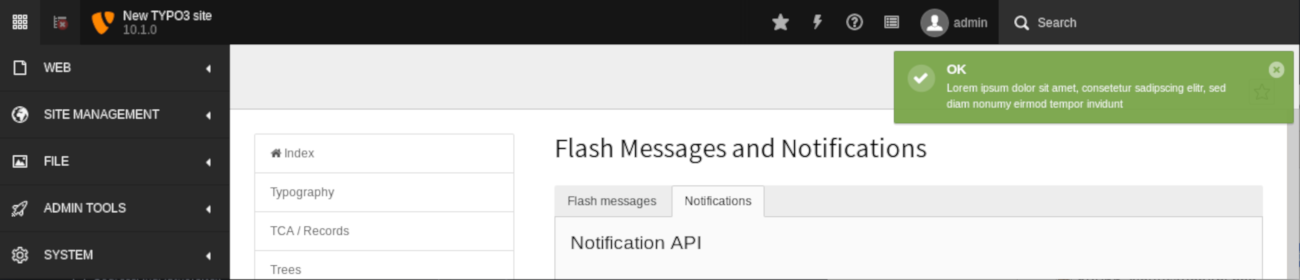
\includegraphics[width=0.90\linewidth]{ChangesForDevelopers/89066-NotificationApi.png}
%	\end{figure}
%
%\end{frame}

% ------------------------------------------------------------------------------
% Feature | 89061 | Introduce Notification Actions

\begin{frame}[fragile]
	\frametitle{In-Depth Changes}
	\framesubtitle{Notification Actions}

	\begin{itemize}
		\item JavaScript notifications in the backend support actions (buttons) now.
	\end{itemize}

	\begin{figure}
		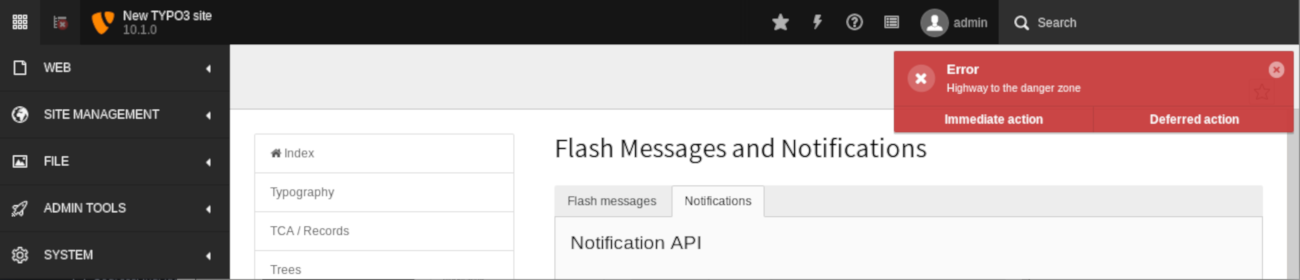
\includegraphics[width=0.90\linewidth]{InDepthChanges/89061-NotificationActionsAndButtons.png}
	\end{figure}

\end{frame}

% ------------------------------------------------------------------------------
% Feature | 89244 | Broadcast Channels and Messaging

\begin{frame}[fragile]
	\frametitle{In-Depth Changes}
	\framesubtitle{Broadcast Channels and Messaging}

	% decrease font size for code listing
	\lstset{basicstyle=\tiny\ttfamily}

	\begin{itemize}
		\item It is now possible to send and receive "broadcast messages" using JavaScript.
	\end{itemize}

	\vspace{-0.2cm}
	\begingroup
		\color{red}
			\begin{center}
				The API is considered \textbf{internal} for the time being\newline
				and may change at any time until declared "stable".
			\end{center}
	\endgroup

	\begin{itemize}
		\item Example for \textbf{sending} a message:
\begin{lstlisting}
require(['TYPO3/CMS/Backend/BroadcastService'], function (BroadcastService) {
  const payload = {
    componentName: 'my_extension',
    eventName: 'my_event',
    foo: 'bar'
  };
  BroadcastService.post(payload);
});
\end{lstlisting}

	\end{itemize}

\end{frame}

% ------------------------------------------------------------------------------
% Feature | 89244 | Broadcast Channels and Messaging

\begin{frame}[fragile]
	\frametitle{In-Depth Changes}
	\framesubtitle{Broadcast Channels and Messaging}

	% decrease font size for code listing
	\lstset{basicstyle=\tiny\ttfamily}

	\begin{itemize}
		\item Example for \textbf{receiving} the message:
\begin{lstlisting}
define([], function() {
  document.addEventListener('typo3:my_component:my_event', (e) => eventHandler(e.detail));
  function eventHandler(detail) {
    // output contains key 'foo' as the payload
    console.log(detail);
  }
});
\end{lstlisting}

		\item See \href{https://developer.mozilla.org/en-US/docs/Web/API/Broadcast_Channel_API}{developer.mozilla.org} for more details.

	\end{itemize}

\end{frame}

% ------------------------------------------------------------------------------
% Feature | 88871 | Handle middleware handler in RequestFactory correctly

\begin{frame}[fragile]
	\frametitle{In-Depth Changes}
	\framesubtitle{RequestFactory Middleware Handler}

	% decrease font size for code listing
	\lstset{basicstyle=\tiny\ttfamily}

	\begin{itemize}
		\item It is now possible to define custom middleware handlers as an array.
		\item The RequestFactory builds a handler stack based on the\newline
			\small
				\texttt{\$GLOBALS['TYPO3\_CONF\_VARS']['HTTP']['handler']}
			\normalsize
			array and injects it into the client.
		\item For example:
\begin{lstlisting}
use \TYPO3\CMS\Core\Utility\GeneralUtility;
use \Vendor\MyExtension\Middleware\Guzzle\CustomMiddleware;
use \Vendor\MyExtension\Middleware\Guzzle\SecondCustomMiddleware;

# Add custom middleware to default Guzzle handler stack
$GLOBALS['TYPO3_CONF_VARS']['HTTP']['handler'][] =
  (GeneralUtility::makeInstance(CustomMiddleware::class))->handler();
$GLOBALS['TYPO3_CONF_VARS']['HTTP']['handler'][] =
  (GeneralUtility::makeInstance(SecondCustomMiddleware::class))->handler();
\end{lstlisting}

	\end{itemize}

\end{frame}

% ------------------------------------------------------------------------------
% Feature | 88602 | Allow registering additional file processors

\begin{frame}[fragile]
	\frametitle{In-Depth Changes}
	\framesubtitle{Custom File Processors}

	% decrease font size for code listing
	\lstset{basicstyle=\tiny\ttfamily}

	\begin{itemize}
		\item Developers can now register their own file processors.
		\item Add the following code to file \texttt{ext\_localconf.php}:
\begin{lstlisting}
$GLOBALS['TYPO3_CONF_VARS']['SYS']['fal']['processors']['ExampleImageProcessor'] = [
  'className' => \Vendor\MyExtension\Resource\Processing\ExampleImageProcessor::class,
  'before' => 'LocalImageProcessor',
];
\end{lstlisting}

		\item Typical use cases:

			\begin{itemize}
				\item add a watermark to images
				\item compress uploaded files to a ZIP archive
				\item store manipulated copies of images
				\item etc.
			\end{itemize}

	\end{itemize}

\end{frame}

% ------------------------------------------------------------------------------
% Feature | 88950 | Add storeSession argument to Widget ViewHelpers

\begin{frame}[fragile]
	\frametitle{In-Depth Changes}
	\framesubtitle{Widget ViewHelpers}

	% decrease font size for code listing
	\lstset{basicstyle=\smaller\ttfamily}

	\begin{itemize}
		\item Widget ViewHelpers set a session cookie in the frontend under certain circumstances.
		\item As this is not always desired (for example due to GDPR), this can be controlled now.
		\item A boolean \texttt{storeSession} has been introduced that lets developers enable/disable this feature.
\begin{lstlisting}
<f:widget.autocomplete
  for="name"
  objects="{posts}"
  searchProperty="author"
  storeSession="false" />
\end{lstlisting}

	\end{itemize}

\end{frame}

% ------------------------------------------------------------------------------
% Feature | 89577 | New PSR-14 based events for File Abstraction Layer
% Deprecation | 89577 | FAL SignalSlot handling migrated to PSR-14 events

\begin{frame}[fragile]
	\frametitle{In-Depth Changes}
	\framesubtitle{PSR-14 Events in FAL}

	% decrease font size for code listing
	\lstset{basicstyle=\tiny\ttfamily}

	\begin{itemize}
		\item Approximately 40 new
			\href{https://www.php-fig.org/psr/psr-14/}{PSR-14}
			based Events have been introduced in the File Abstraction Layer (FAL).
		\item They replace existing Extbase Signal/Slots.
		\item Using the Signals continues to work (without producing any deprecation message!).
			However, the Signals in the FAL will likely be removed in TYPO3 v11.
		\item Extension authors are advised to migrate their code and use Events.
		\item Review the new PHP classes to learn more about PSR-14.
	\end{itemize}

\end{frame}


% ------------------------------------------------------------------------------
% Deprecation | 89733 | Signal Slots in Core Extension migrated to PSR-14 events

\begin{frame}[fragile]
	\frametitle{In-Depth Changes}
	\framesubtitle{PSR-14 Events in the TYPO3 Core}

	\begin{itemize}
		\item A number of new PSR-14 Events replace Signal/Slots in the TYPO3 core:
			\newline

			\begin{itemize}\tiny
				\item \texttt{TYPO3\textbackslash
					CMS\textbackslash
					Core\textbackslash
					Imaging\textbackslash
					Event\textbackslash
					ModifyIconForResourcePropertiesEvent}
					\newline
				\item \texttt{TYPO3\textbackslash
					CMS\textbackslash
					Core\textbackslash
					DataHandling\textbackslash
					Event\textbackslash
					IsTableExcludedFromReferenceIndexEvent}
					\newline
				\item \texttt{TYPO3\textbackslash
					CMS\textbackslash
					Core\textbackslash
					DataHandling\textbackslash
					Event\textbackslash
					AppendLinkHandlerElementsEvent}
					\newline
				\item \texttt{TYPO3\textbackslash
					CMS\textbackslash
					Core\textbackslash
					Configuration\textbackslash
					Event\textbackslash
					AfterTcaCompilationEvent}
					\newline
				\item \texttt{TYPO3\textbackslash
					CMS\textbackslash
					Core\textbackslash
					Database\textbackslash
					Event\textbackslash
					AlterTableDefinitionStatementsEvent}
					\newline
				\item \texttt{TYPO3\textbackslash
					CMS\textbackslash
					Core\textbackslash
					Tree\textbackslash
					Event\textbackslash
					ModifyTreeDataEvent}
					\newline
				\item \texttt{TYPO3\textbackslash
					CMS\textbackslash
					Backend\textbackslash
					Backend\textbackslash
					Event\textbackslash
					SystemInformationToolbarCollectorEvent}
					\newline
			\end{itemize}

	\end{itemize}

\end{frame}

% ------------------------------------------------------------------------------
% Deprecation | 89718 | Legacy PageTSconfig parsing lowlevel API

\begin{frame}[fragile]
	\frametitle{In-Depth Changes}
	\framesubtitle{TSconfig Parsing}

	% decrease font size for code listing
	\lstset{basicstyle=\tiny\ttfamily}

	\begin{itemize}
		\item Two new PHP classes have been introduced to load and parse PageTSconfig:
			\begin{itemize}\smaller
				\item \texttt{TYPO3\textbackslash
					CMS\textbackslash
					Core\textbackslash
					Configuration\textbackslash
					Loader\textbackslash
					PageTsConfigLoader}
				\item \texttt{TYPO3\textbackslash
					CMS\textbackslash
					Core\textbackslash
					Configuration\textbackslash
					Parser\textbackslash
					PageTsConfigParser}
			\end{itemize}

		\item For example:
\begin{lstlisting}
// Fetch all available PageTS of a page/rootline:
$loader = GeneralUtility::makeInstance(PageTsConfigLoader::class);
$tsConfigString = $loader->load($rootLine);

// Parse the string and apply conditions:
$parser = GeneralUtility::makeInstance(
  PageTsConfigParser::class, $typoScriptParser, $hashCache
);

$pagesTSconfig = $parser->parse($tsConfigString, $conditionMatcher);
\end{lstlisting}

	\end{itemize}

\end{frame}

% ------------------------------------------------------------------------------
% Important | 87518 | Use prepared statements for pdo_mysql per default

\begin{frame}[fragile]
	\frametitle{In-Depth Changes}
	\framesubtitle{Prepared Statements}

	% decrease font size for code listing
	\lstset{basicstyle=\tiny\ttfamily}

	\begin{itemize}
		\item The \texttt{pdo\_mysql} driver uses prepared statements by default now.
		\item In older versions of TYPO3, \textit{emulated prepared statements} were used.
			This means, all returned values of a query were strings.
		\item This behavior has changed and prepared statements are used
			which return native data types.
		\item For example: values of a column defined as integer are returned in PHP as \texttt{int}.
		\item This feature can be deactivated by setting the option
			\texttt{PDO::ATTR\_EMULATE\_PREPARES} in your database connection.

	\end{itemize}

\end{frame}

% ------------------------------------------------------------------------------
% Feature | 87380 | Introduce SiteLanguageAwareInterface to denote site language awareness

\begin{frame}[fragile]
	\frametitle{In-Depth Changes}
	\framesubtitle{Denote Site Language Awareness}

	% decrease font size for code listing
	\lstset{basicstyle=\tiny\ttfamily}

% A SiteLanguageAwareInterface with the methods setSiteLanguage(Entity\SiteLanguage $siteLanguage) and getSiteLanguage() has been introduced.
% The interface can be used to denote a class as aware of the site language.

	\begin{itemize}
		\item A \texttt{SiteLanguageAwareInterface} has been introduced.
		\item The interface can be used to denote a class as aware of the site language.
		\item Routing aspects, that take the site language into account,
			are now using the \texttt{SiteLanguageAwareInterface}
			in addition to the \texttt{SiteLanguageAwareTrait}.
	\end{itemize}

\end{frame}

% ------------------------------------------------------------------------------
% Important | 89645 | Removed systemLog options

\begin{frame}[fragile]
	\frametitle{In-Depth Changes}
	\framesubtitle{System Log API}

	% decrease font size for code listing
	\lstset{basicstyle=\tiny\ttfamily}

	\begin{itemize}
		\item The following options have been removed from TYPO3's default configuration:

			\begin{itemize}\smaller
				\item \texttt{\$GLOBALS['TYPO3\_CONF\_VARS']['SYS']['systemLog']}
				\item \texttt{\$GLOBALS['TYPO3\_CONF\_VARS']['SYS']['systemLogLevel']}
			\end{itemize}\normalsize

		\item Extension authors are adviced to use the Logging API and remove the systemLog options.
	\end{itemize}

\end{frame}

% ------------------------------------------------------------------------------
% Feature | 89603 | Introduce native pagination for lists

\begin{frame}[fragile]
	\frametitle{In-Depth Changes}
	\framesubtitle{Native List Pagination}

	% decrease font size for code listing
	\lstset{basicstyle=\tiny\ttfamily}

	\begin{itemize}
		\item Native support for the pagination of lists such as arrays or QueryResults of Extbase has been introduced.
		\item The \texttt{PaginatorInterface} defines a basic set of methods.
		\item The \texttt{AbstractPaginator} class holds the main pagination logic.
		\item This enables developers to implement all kinds of paginators.
\begin{lstlisting}
use TYPO3\CMS\Core\Pagination\ArrayPaginator;

$items = ['apple', 'banana', 'strawberry', 'raspberry', 'ananas'];
$currentPageNumber = 3;
$itemsPerPage = 2;

$paginator = new ArrayPaginator($itemsToBePaginated, $currentPageNumber, $itemsPerPage);
$paginator->getNumberOfPages(); // returns 3
$paginator->getCurrentPageNumber(); // returns 3
$paginator->getKeyOfFirstPaginatedItem(); // returns 5
$paginator->getKeyOfLastPaginatedItem(); // returns 5
\end{lstlisting}

	\end{itemize}

\end{frame}

% ------------------------------------------------------------------------------
% Deprecation | 89579 | ServiceChains require an array for excluded Service keys

\begin{frame}[fragile]
	\frametitle{In-Depth Changes}
	\framesubtitle{Service API}

	\begin{itemize}
		\item Argument \texttt{\$excludeServiceKeys} is used for skipping certain services when using a chain.
		\item The argument has been changed from a comma-separated list to an array.
		\item This change affects the Service API within the following components:

			\begin{itemize}
				\item \texttt{GeneralUtility::makeInstanceService()}
				\item \texttt{ExtensionManagementUtility::findService()}
			\end{itemize}

		\item Passing a comma-separated list still works but has been marked as \textbf{deprecated}.

	\end{itemize}

\end{frame}

% ------------------------------------------------------------------------------
% Feature | 86614 | Add PSR-14 event to control hreflang tags to be rendered

\begin{frame}[fragile]
	\frametitle{In-Depth Changes}
	\framesubtitle{Modify \texttt{hreflang}-tag}

	% decrease font size for code listing
	\lstset{basicstyle=\smaller\ttfamily}

	\begin{itemize}
		\item It is now possible to modify \texttt{hreflang} tags before they get rendered.
		\item Developers can achieve this by registering an event listener for the following event:\newline
			\smaller
				\texttt{TYPO3\textbackslash
					CMS\textbackslash
					Frontend\textbackslash
					Event\textbackslash
					ModifyHrefLangTagsEvent}
			\normalsize
	\end{itemize}

\end{frame}

% ------------------------------------------------------------------------------
% Feature | 88818 | Introduce events to modify CKEditor configuration

\begin{frame}[fragile]
	\frametitle{In-Depth Changes}
	\framesubtitle{Modify the CKEditor Configuration}

	% decrease font size for code listing
	\lstset{basicstyle=\tiny\ttfamily}

	\begin{itemize}
		\item The following PSR-14-based events have been introduced which allow to modify the CKEditor configuration:
\begin{lstlisting}
TYPO3\CMS\RteCKEditor\Form\Element\Event\AfterGetExternalPluginsEvent
TYPO3\CMS\RteCKEditor\Form\Element\Event\BeforeGetExternalPluginsEvent
TYPO3\CMS\RteCKEditor\Form\Element\Event\AfterPrepareConfigurationForEditorEvent
TYPO3\CMS\RteCKEditor\Form\Element\Event\BeforePrepareConfigurationForEditorEvent
\end{lstlisting}

		\item The
			\href{https://docs.typo3.org/c/typo3/cms-core/master/en-us/Changelog/10.3/Feature-88818-IntroduceEventsToModifyCKEditorConfiguration.html}{change log}
			for an example.
	\end{itemize}

\end{frame}

% ------------------------------------------------------------------------------
% Feature | 89738 | API for AJAX Requests

\begin{frame}[fragile]
	\frametitle{In-Depth Changes}
	\framesubtitle{API for AJAX Requests}

	% decrease font size for code listing
	\lstset{basicstyle=\tiny\ttfamily}

	\begin{itemize}
		\item The \textbf{Fetch API} has been introduced to perform AJAX requests
			and to make TYPO3 less dependent on jQuery.
		\item The API provides a generic definition of Request and Response objects
			(and other things involved with network requests).
		\item Supported by all modern browsers, see
			\href{https://developer.mozilla.org/en-US/docs/Web/API/Fetch_API}{compatibility chart}.
		\item The TYPO3 core uses the new API in the Install Tool, FormEngine, and
			context menus already.
		\item See the
			\href{https://docs.typo3.org/c/typo3/cms-core/master/en-us/Changelog/10.3/Feature-89738-ApiForAjaxRequests.html}{change log}
			for some examples on how to use the Fetch API.

	\end{itemize}

\end{frame}

% ------------------------------------------------------------------------------
% Feature | 89650 | Allow line breaks in TCA descriptions

\begin{frame}[fragile]
	\frametitle{In-Depth Changes}
	\framesubtitle{TCA Description Fields}

	\begin{itemize}
		\item The description field in the TCA can now contain line breaks to make long texts more readable.
	\end{itemize}

\end{frame}

% ------------------------------------------------------------------------------
% Important | 90020 | Legacy BasicFileUtility and ExtendedFileUtility classes marked as internal

\begin{frame}[fragile]
	\frametitle{In-Depth Changes}
	\framesubtitle{Classes \texttt{BasicFileUtility} and \texttt{ExtendedFileUtility}}

	\begin{itemize}
		\item The following two legacy classes have been marked as \textbf{internal}
			and should not be used anymore:

			\begin{itemize}\small
				\item \texttt{TYPO3\textbackslash
					CMS\textbackslash
					Core\textbackslash
					Utility\textbackslash
					File\textbackslash
					BasicFileUtility}
				\item \texttt{TYPO3\textbackslash
					CMS\textbackslash
					Core\textbackslash
					Utility\textbackslash
					File\textbackslash
					ExtendedFileUtility}
			\end{itemize}

		\item Extension developers should use the classes \texttt{ResourceStorage}
			and \texttt{ResourceFactory} for managing assets instead.

	\end{itemize}

\end{frame}

% ------------------------------------------------------------------------------
% Feature | 89139 | Add dependency injection support for console commands

\begin{frame}[fragile]
	\frametitle{In-Depth Changes}
	\framesubtitle{Console Commands: Symfony DI Support}

	\begin{itemize}
		\item Command dependencies can now be injected via constructor or other injection techniques.
		\item Add the \texttt{console.command} tag to command classes.
		\item Use the tag attribute \texttt{command} to specify the command name.
		\item The optional tag attribute \texttt{schedulable} can be set to \texttt{false}
			to exclude the command from the TYPO3 scheduler.

		\item See
			\href{https://docs.typo3.org/c/typo3/cms-core/master/en-us/Changelog/10.3/Feature-89139-AddDependencyInjectionSupportForConsoleCommands.html}{change log}
			for an example.
	\end{itemize}

\end{frame}

% ------------------------------------------------------------------------------
% Feature | 90168 | Introduce Modal Actions

\begin{frame}[fragile]
	\frametitle{In-Depth Changes}
	\framesubtitle{Action Buttons in Modals}

	% decrease font size for code listing
	\lstset{basicstyle=\tiny\ttfamily}

	\begin{itemize}
		\item Modal popups now support action buttons.
		\item As an alternative to the existing \texttt{trigger} option, the new option
			\texttt{action} can be used.
		\item For example:
\begin{lstlisting}
Modal.confirm('Header', 'Some content', Severity.error, [
  {
    text: 'Based on trigger()',
    trigger: function () {
      console.log('Vintage!');
    }
  },
  {
    text: 'Based on action()',
    action: new DeferredAction(() => {
      return new AjaxRequest('/any/endpoint').post({});
    })
  }
]);
\end{lstlisting}

	\end{itemize}

\end{frame}

% ------------------------------------------------------------------------------
% Feature | 90471 | JavaScript Event API

\begin{frame}[fragile]
	\frametitle{In-Depth Changes}
	\framesubtitle{JavaScript Event API}

	\begin{itemize}
		\item A new Event API enables JavaScript developers to have a stable event listening interface.
		\item The API takes care of common pitfalls like event delegation and clean event unbinding.
		\item Each \textit{event strategy} offers two ways to bind a listener to an event.
		\item The Event API offers several strategies to handle event listeners.
		\item See
			\href{https://docs.typo3.org/c/typo3/cms-core/master/en-us/Changelog/10.3/Feature-90471-JavaScriptEventAPI.html}{change log}
			for examples and further details.
	\end{itemize}

\end{frame}

% ------------------------------------------------------------------------------
% Feature | 88648 | Define Twitter Card Type In Page Properties
% Important | 86577 | Query parameters are now included in canonicalized URLs

\begin{frame}[fragile]
	\frametitle{In-depth Changes}
	\framesubtitle{Miscellaneous}

	% decrease font size for code listing
	\lstset{basicstyle=\tiny\ttfamily}

	\begin{itemize}

		\item Type of Twitter Card can be selected/configured now.
			This option renders the meta tag \texttt{twitter:card} in the frontend.
\begin{lstlisting}
page {
  meta {
    twitter:card = summary_large_image
    twitter:card.replace = 1
  }
}
\end{lstlisting}

		\item Only parameters that are needed to calculate the cHash are included in canonicalized URLs by default.
			Additional query parameters can now be configured:
\begin{lstlisting}
$GLOBALS['TYPO3_CONF_VARS']['FE']['additionalCanonicalizedUrlParameters'].
\end{lstlisting}

		\smaller
			Note: only add parameters which change the content of your page. Otherwise search engines will likely classify your pages as duplicate content.
		\normalsize

	\end{itemize}

\end{frame}

% ------------------------------------------------------------------------------
% Breaking | 88681 | Import Of PHP Files In Import Export Files Removed
% Breaking | 88500 | RTE image handling functionality dropped
% Breaking | 81950 | Remove leftover workspaces unpublishing functionality

\begin{frame}[fragile]
	\frametitle{In-depth Changes}
	\framesubtitle{Miscellaneous}

	% decrease font size for code listing
	\lstset{basicstyle=\tiny\ttfamily}

	\begin{itemize}

		\item When importing XML data using \texttt{EXT:impexp}, the File Deny Pattern applies
			now and rejects embedded PHP files for example.

		\item RTE image handling functionality has been removed completely.
			For image support in CKEditor, consider to use \texttt{EXT:rte\_ckeditor\_image} for example.

		\item A property within workspaces for \textit{unpublishing} records has been removed in v10
			(including the database field \texttt{sys\_workspace.unpublish\_time}). This feature was
			disabled in TYPO3 v4.5 and not used or provided by the TYPO3 core.

	\end{itemize}

\end{frame}

% ------------------------------------------------------------------------------
% Breaking | 88772 | JavaScript script tags omit type=text/javascript in HTML5
% Remove system extension EXT:rsaauth
% Remove system extension EXT:fe_edit

\begin{frame}[fragile]
	\frametitle{In-depth Changes}
	\framesubtitle{Miscellaneous}

	% decrease font size for code listing
	\lstset{basicstyle=\tiny\ttfamily}

	\begin{itemize}

		\item When rendering HTML5 output, \texttt{<script>} tags do not include
			the attribute \texttt{type="text/javascript"} anymore.

		\item This can be re-enabled for the frontend by using TypoScript if required:
\begin{lstlisting}
page {
  includeJS {
    myfile = EXT:example/Resources/Public/JavaScript/myfile.js
    myfile.type = text/javascript
  }
}
\end{lstlisting}

		\item The following deprecated system extensions have been removed:

			\begin{itemize}
				\item \texttt{EXT:rsaauth}
				\item \texttt{EXT:fe\_edit}
			\end{itemize}

	\end{itemize}

\end{frame}

% ------------------------------------------------------------------------------
% Breaking | 88525 | Remove “createDirs” directive of extension installation / ext_emconf.php
% Breaking | 87511 | Remove $viewFormatToObjectNameMap property
% Breaking | 87511 | Remove $namespacesViewObjectNamePattern property
% Feature | 87726 | Extend Frontend Login Controller Hook To Validate Password

\begin{frame}[fragile]
	\frametitle{In-Depth Changes}
	\framesubtitle{Miscellaneous}

	\begin{itemize}
		\item Directive \texttt{createDirs} in file \texttt{ext\_emconf.php} not supported anymore.

			\begin{itemize}\smaller
				\item[\ding{228}] Folders will not be created automatically during extension installation.
			\end{itemize}\normalsize

		\item The following two properties in class
			\texttt{TYPO3\textbackslash
				CMS\textbackslash
				Extbase\textbackslash
				Mvc\textbackslash
				Controller\textbackslash
				ActionController}\newline
			have been removed:

			\begin{itemize}
				\item \texttt{\$namespacesViewObjectNamePattern}
				\item \texttt{\$viewFormatToObjectNameMap}
			\end{itemize}

		\item The following existing hook has been extended and can now
			also be used to validate passwords:\newline
			{\fontsize{8}{10} \selectfont \texttt{\$GLOBALS['TYPO3\_CONF\_VARS']['EXTCONF']['felogin']['password\_changed']}}

	\end{itemize}

\end{frame}

% ------------------------------------------------------------------------------
% Deprecation | 87613 | Deprecate /TYPO3/CMS/Extbase/Utility/TypeHandlingUtility::hex2bin
% Deprecation | 88554 | Deprecated methods in VersionNumberUtility

\begin{frame}[fragile]
	\frametitle{In-Depth Changes}
	\framesubtitle{Miscellaneous}

	\begin{itemize}

		\item The following methods of class
			\smaller\texttt{\textbackslash
				TYPO3\textbackslash
				CMS\textbackslash
				Core\textbackslash
				Utility\textbackslash
				VersionNumberUtility}\normalsize\newline
			have been marked deprecated:

			\begin{itemize}
				\item \texttt{convertIntegerToVersionNumber()}
				\item \texttt{splitVersionRange()}
				\item \texttt{raiseVersionNumber()}
			\end{itemize}

			\begin{itemize}\smaller
				\item[\ding{228}] Implement the methods as custom code.
			\end{itemize}\normalsize

	\end{itemize}

\end{frame}

% ------------------------------------------------------------------------------
% Feature | 86964 | Allow getting class property default value
% Deprecation | 82669 | Streamline Backend route path inconsistencies

\begin{frame}[fragile]
	\frametitle{In-Depth Changes}
	\framesubtitle{Miscellaneous}

	% decrease font size for code listing
	\lstset{basicstyle=\tiny\ttfamily}

	\begin{itemize}
		\item It is now possible to get the default value of a class property
			when using the ReflectionService.
\begin{lstlisting}
$property = GeneralUtility::makeInstance(ReflectionService::class)
  ->getClassSchema(MyClass::class)
  ->getProperty('myProperty');
\end{lstlisting}

		\item Backend routes to modules without path configurations are now named\newline
			"\texttt{/module/<main-module>/<sub-module>}" by default\newline
			\small
				(for example: "\texttt{/module/web/ts}".)
			\normalsize

		\item Old routes still work (e.g. "\texttt{/web/ts/}") but this syntax will be removed in TYPO3 v11.

	\end{itemize}

\end{frame}

% ------------------------------------------------------------------------------
% Breaking | 88669 | FormEngine FormDataProvider parentPageTca removed
% Breaking | 88744 | Database fields related to CSS Styled Content removed
% Breaking | 88143 | Version-related database field “t3ver_id” removed
% Deprecation | 88746 | PageRepository PHP class moved from Frontend to Core Extension

\begin{frame}[fragile]
	\frametitle{In-Depth Changes}
	\framesubtitle{Miscellaneous}

	\begin{itemize}
		\item The FormEngine DataProvider \texttt{parentPageTca} has been removed.

			\begin{itemize}\smaller
				\item[\ding{228}] Developers can access \texttt{\$GLOBALS['TCA']['pages']} directly, instead of \texttt{\$result['parentPageTca']}.
			\end{itemize}\normalsize

		\item The following database fields have been removed:

			\begin{itemize}\smaller
				\item \texttt{tt\_content.spaceBefore} (replaced by field \texttt{space\_before\_class})
				\item \texttt{tt\_content.spaceAfter} (replaced by field \texttt{space\_after\_class})
				\item \texttt{pages.t3ver\_id} (unused since TYPO3 v9)
			\end{itemize}\normalsize

		\item The PHP class
			\texttt{\textbackslash
				TYPO3\textbackslash
				CMS\textbackslash
				Frontend\textbackslash
				Page\textbackslash
				PageRepository} has been moved from the "frontend" system extension into the core.

			\begin{itemize}\smaller
				\item Replace with class:
					\texttt{\textbackslash
						TYPO3\textbackslash
						CMS\textbackslash
						Core\textbackslash
						Domain\textbackslash
						Repository\textbackslash
						PageRepository}
			\end{itemize}\normalsize

	\end{itemize}

\end{frame}

% ------------------------------------------------------------------------------
% Breaking | 88574 | 4th parameter of PageRepository>enableFields removed
% Deprecation | 85895 | Deprecate File::_getMetaData()
% Deprecation | 88662 | Deprecated backend route xMOD_tximpexp

\begin{frame}[fragile]
	\frametitle{In-Depth Changes}
	\framesubtitle{Miscellaneous}

	\begin{itemize}

		\item 4th parameter of method \texttt{PageRepository->enableFields()} has been removed.

		\begin{itemize}\smaller
			\item[\ding{228}] If developers use a 4th parameter in this method call, which is set to "\textbf{false}", this can be removed safely.
			\item[\ding{228}] If it is set to "\textbf{true}", the code needs to be replaced with a separate instance of \texttt{PageRepository} with a custom \texttt{Context}.
		\end{itemize}\normalsize

		\item The internal method \texttt{File::\_getMetaData()}, which is used to fetch meta data of a file,
			has been marked deprecated.

			\begin{itemize}\smaller
				\item[\ding{228}] Use \texttt{\$fileObject->getMetaData()->get()} to fetch the meta data instead.
			\end{itemize}\normalsize

		\item The route identifier "\texttt{xMOD\_tximpexp}" has been marked deprecated.

			\begin{itemize}\smaller
				\item[\ding{228}] Use \texttt{tx\_impexp\_export} or \texttt{tx\_impexp\_import} depending on the use case.
			\end{itemize}\normalsize

	\end{itemize}

\end{frame}

% ------------------------------------------------------------------------------
% Breaking | 88496 | Method getSwitchableControllerActions has been removed
% Breaking | 87567 | Global variable $TBE_TEMPLATE removed
% Breaking | 88660 | $GLOBALS[T3_VAR] removed

\begin{frame}[fragile]
	\frametitle{In-Depth Changes}
	\framesubtitle{Miscellaneous}

	\begin{itemize}

		\item The following abstract method has been removed:\newline
			\smaller
				\texttt{\textbackslash
					TYPO3\textbackslash
					CMS\textbackslash
					Extbase\textbackslash
					Configuration\textbackslash
					AbstractConfigurationManager::}\newline
					\texttt{getSwitchableControllerActions()}
			\normalsize

			\begin{itemize}\smaller
				\item[\ding{228}] Use the new method name \texttt{getControllerConfiguration()} instead (same PHP class).
			\end{itemize}\normalsize

		\item The global variable \texttt{\$TBE\_TEMPLATE} has been removed, including
			the related PSR-15 middleware (which was marked as internal).

			\begin{itemize}\smaller
				\item[\ding{228}] Instantiate the DocumentTemplate class directly in the controller of the module.
				\item[\ding{228}] Migrate to ModuleTemplate which is available since TYPO3 v7.
			\end{itemize}\normalsize

		\item The global variable \texttt{\$GLOBALS['T3\_VAR']} has been removed.\newline

	\end{itemize}

\end{frame}

% ------------------------------------------------------------------------------
% Important | 89001 | TSFE->createHashBase
% Feature | 89150 | Add events before and after rollback of record history entries

\begin{frame}[fragile]
	\frametitle{In-Depth Changes}
	\framesubtitle{Miscellaneous}

	\begin{itemize}
		\item The \texttt{hashParameters} for calculating the hashBase in the following class have been modified:\newline
			\small
				\texttt{TYPO3\textbackslash
					CMS\textbackslash
					Frontend\textbackslash
					Controller\textbackslash
					TypoScriptFrontendController}
			\normalsize

			\begin{itemize}
				\item \texttt{gr\_list} has been replaced by \texttt{groupIds}.
				\item \texttt{cHash} has been replaced by \texttt{dynamicArguments}.
				\item \texttt{domainStartPage} has been replaced by \texttt{site} (site identifier).
			\end{itemize}

		\item Two new events are dispatched when records are rolled back:

			\begin{itemize}\smaller
				\item \texttt{TYPO3\textbackslash
					CMS\textbackslash
					Backend\textbackslash
					History\textbackslash
					Event\textbackslash
					BeforeHistoryRollbackStartEvent}
				\item \texttt{TYPO3\textbackslash
					CMS\textbackslash
					Backend\textbackslash
					History\textbackslash
					Event\textbackslash
					AfterHistoryRollbackFinishedEvent}
			\end{itemize}\normalsize

	\end{itemize}

\end{frame}

% ------------------------------------------------------------------------------
% Feature | 88805 | Add type to TYPO3/CMS/Core/Database/Query/QueryBuilder::set()

\begin{frame}[fragile]
	\frametitle{In-Depth Changes}
	\framesubtitle{Miscellaneous}

	\begin{itemize}
		\item Method \texttt{set()} of the Query Builder now accepts a 4th argument
			to specify the type of the named parameter:\newline
			\small
				\texttt{TYPO3\textbackslash
					CMS\textbackslash
					Core\textbackslash
					Database\textbackslash
					Query\textbackslash
					QueryBuilder::set()}
			\normalsize\newline
			\vspace{0.2cm}
			(the default is \texttt{\textbackslash PDO::PARAM\_STR})

	\end{itemize}

\end{frame}

% ------------------------------------------------------------------------------
% Feature | 21638 | Introduced IP locking for IPv6
% Breaking | 21638 | AbstractUserAuthentication::lockIP property removed

\begin{frame}[fragile]
	\frametitle{In-depth Changes}
	\framesubtitle{Miscellaneous}

	% decrease font size for code listing
	\lstset{basicstyle=\tiny\ttfamily}

	\begin{itemize}

		\item  The IP locking functionality has been extended to also support IPv6
			(frontend and backend).
\begin{lstlisting}
$GLOBALS['TYPO3_CONF_VARS']['FE']['lockIPv6'] = 2;
$GLOBALS['TYPO3_CONF_VARS']['BE']['lockIPv6'] = 2;
\end{lstlisting}

		\item The public property \texttt{lockIP} in following PHP class has been removed:\newline
			\small
				\texttt{\textbackslash
					TYPO3\textbackslash
					CMS\textbackslash
					Core\textbackslash
					Authentication\textbackslash
					AbstractUserAuthentication}.
			\normalsize

		\item Migration options:

			\begin{itemize}\smaller
				\item[\ding{228}] Set \texttt{lockIP} and \texttt{lockIPv6} in \texttt{\$GLOBALS['TYPO3\_CONF\_VARS'][...]}.
				\item[\ding{228}] Use the new IP-Locker API:
					\texttt{\textbackslash
						TYPO3\textbackslash
						CMS\textbackslash
						Core\textbackslash
						Authentication\textbackslash
						IpLocker}.
			\end{itemize}\normalsize

	\end{itemize}

\end{frame}

% ------------------------------------------------------------------------------
